\documentclass[11pt]{article}

\renewcommand{\baselinestretch}{1.1}
%\usepackage[scaled]{helvet}
%\renewcommand{\familydefault}{\sfdefault}
\usepackage{amssymb,amsmath,amsthm}
\usepackage{graphicx}
\usepackage{caption}
\usepackage{subfig}
\usepackage{wrapfig}
\usepackage{framed}
\usepackage{tikz}
\usepackage{mathrsfs}
\usepackage{enumerate}

%\usepackage{subcaption}


\pagestyle{plain}

\setlength{\oddsidemargin}{-5mm}
\addtolength{\textwidth}{4.5cm}
\addtolength{\textheight}{4.cm}
\setlength{\topmargin}{-2cm}
\setlength{\parskip}{4pt}
\setlength{\parindent}{0pt}


\setlength{\unitlength}{1in}
\renewcommand{\baselinestretch}{1.1}



%
%\usepackage{geometry}                % See geometry.pdf to learn the layout options. There are lots.
%\geometry{letterpaper}   
%\usepackage{amsmath}                % ... or a4paper or a5paper or ... 
%%\geometry{landscape}                % Activate for for rotated page geometry
%%\usepackage[parfill]{parskip}    % Activate to begin paragraphs with an empty line rather than an indent
%\usepackage{graphicx}
%\usepackage{amssymb}
%\usepackage{epstopdf}


\newcommand{\eps}{\varepsilon}
\newcommand{\rmO}{\mathrm{O}}
\newcommand{\rmo}{\mathrm{o}}
\newcommand{\rmspan}{\mathrm{span}}
\newcommand{\rmd}{\mathrm{d}}
\newcommand{\rme}{\mathrm{e}}
\newcommand{\rmi}{\mathrm{i}}
\newcommand{\R}{\mathbb{R}}
\newcommand{\C}{\mathbb{C}}
\newcommand{\N}{\mathbb{N}}
\usepackage{amsthm}
\theoremstyle{plain}

\newtheorem{Lemma}{Lemma}[section]
\newtheorem*{Lemma*}{Lemma}
\newtheorem{Theorem}{Theorem}
\newtheorem*{Theorem*}{Theorem}
\newtheorem{Proposition}[Lemma]{Proposition}
\newtheorem*{Proposition*}{Proposition}
\newtheorem{Corollary}[Lemma]{Corollary}
\newtheorem{Remark}[Lemma]{Remark}
\newtheorem{Definition}[Lemma]{Definition}
\newtheorem{Hypothesis}[Lemma]{Hypothesis}
\newtheorem*{Hypothesis*}{Hypothesis}




\DeclareGraphicsRule{.tif}{png}{.png}{`convert #1 `dirname #1`/`basename #1 .tif`.png}

\title{Modified Split Bregman}
\author{Gabriela Jaramillo and Shankar Venkataramani}
%\date{}                                           % Activate to display a given date or no date

\begin{document}
\maketitle

\begin{abstract}
The goal of this paper is to describe the microstructures that emerge when one seeks to minimize nonconvex energies. In particular we consider functionals that are defined over real valued functions and that are nonconvex in both the variable and its gradient. To  characterize these microstructures we minimize the associated relaxed problem using two novel approaches: i) a semi-analytical method based on Control Systems Theory, ii) and a numerical scheme that combines convex splitting together with a modified version of the Split Bregman algorithm. These solutions are then used to gain information about minimizing sequences of the original problem. In particular we describe how to recover the location and length scale of oscillations.
\end{abstract}

%%%%%%%%%%%%%%%%%%%%%%%%%%%%%%%%%%%%%%%%%%%%%%%%%%%%%%%%%%%%%%%%
%%%%%%%%%%%%%%%%%%%%%%%%% INTRODUCTION %%%%%%%%%%%%%%%%%%%%%%%%%%%
\section{Introduction}\label{s:intro}


In this paper we consider the following problem,
\begin{equation}\label{e:original}
 \min_A I[u] = \min_A \int_a^b W(u_x) + V(x,u) \;dx \hspace{1.5cm} u \in A
 \end{equation}
where $W(\xi)$ is a nonconvex potential, $V(x,u)$ a continuous function, and $u$ is a real valued function living in an appropriate space, which we denote here by $A$. As is well known, the lack of convexity implies that the functional, $I[u]$, is not weakly lower semicontinuous. Therefore, the Direct Method of the Calculus of Variations cannot be applied and a classical solution to this minimization problem cannot be found. At the same time, minimizing sequences are characterized by finite amplitude fine scale oscillations, which in applications correspond to the emergence of microstructures. Examples of systems that exhibit this behavior are: solid materials like steel where microstructures appear in the form of phase transitions, plastically deformed crystals and their dislocation patterns, and biological materials like leafs and the ripples present on their edges , to name just a few examples. Our goal in this paper is to understand microstructures in the context of problems of the form \eqref{e:original}, and to provide a methodology for characterizing their location and length scale. 

A classical approach for understanding the oscillations that are present in  minimizing sequences is through the theory of Young's measures. Given that the original problem does not posses minimizers in the classical sense, Young's measures enlarge the set of admissible solutions to include those that can be described by probability measures. The oscillations, which in the present case can be interpret as the system selecting a solution out of a discrete set with a certain probability, are described precisely by these measures. This leads to a generalized functional, $\tilde{I}[\mu]$, whose infimum under certain assumptions coincides with that of the relaxation of the original problem. 
  
Another approach for dealing with nonconvex energies is to incorporate higher order terms in order to regularize the functional.  In other words, regularizing consists in adding to the energy terms that would normally be ignored because they are small, but that are necessary in order to capture the small scale behavior of solutions.  For example, in exploring wrinkling in thin elastic sheets one seeks to minimize a nonconvex strain energy that depends on the gradients of the deformation, plus a small perturbation that depends on the hessian of the deformation and that represents the bending energy. In very broad terms, this perturbation acts as a selection mechanisms that allows one to determine the length scale of these wrinkles. In this example, as well as in other applications, the difficulty is that finding minimizers for the regularized functional, either by solving the Euler Lagrange equations or through computaitonal methods, is extremely difficult. This issue can in part be resolved if one considers instead the family of functionals parametrized by the perturbation and the corresponding  $\Gamma$-limit as this parameter (which we denote by $\eps$) goes to zero. The idea being that the limiting problem retains enough information about the original problem while at the same time being much easier to solve. An important aspect of the examples considered here is that their regularization $\Gamma$-converges to the relaxation of the original problem.

The ideas presented above can be summarized in the following diagram, showing a connection between the the regularization of the original problem, $I^\eps[u]$, its generalization via Young measures, $\tilde{I}[u]$, and its relaxation, $\overline{I}[u]$.

 
 \vspace{4ex}
\begin{center}
\begin{tikzpicture}
\node [left] at (0,0) {$I[u]$};
\draw [thick, ->] (0,0.1) --(2.5,1);
\node [right] at (2.5,1) {$I^\eps[u]$};
\draw [thick, ->] (3.5,1) --(6,0.1);
\node [right] at (6,0) {$\overline{I}[u]$};
\draw [thick, ->] (0,-0.1) --(2.5,-1);
\node [right] at (2.5,-1) {$\tilde{I}[u]$};
\draw [thick, ->] (3.5,-1) --(6,-0.1);
\node [rotate=20] at (0.9,0.9) {Regularize};
\node [rotate=-20] at (0.9,-0.9) {Generalize};
\node [rotate=-20] at (4.5,1) {$\Gamma$-limit};
\node [rotate=20] at (4.5,-1) {Relax};
\end{tikzpicture}
\end{center}
  The key point is that for the functionals considered in this paper the relaxation, $\overline{I}[u]$, corresponds to the convexification of $I[u]$ in the gradient variable, $u_x$. Moreover, minimizers of the relaxation  exist and carry information about  the optimal measure that minimizes $\tilde{I}[\mu]$. As a result, these solutions also provide information about the minimizing sequences of the original functional. In particular, one can use the minimizer of the relaxation to infer the location of fine scaled oscillations. On the other hand, the relaxation also corresponds to the $\Gamma$-limit of the family of regularized problems, allowing us to infer the scale of oscillations in terms of $\eps$, the scale of the perturbation. This is done by assuming an equipartition of the energy and using a scaling argument.
  

These observations provide a strong motivation for studying minimizers of the relaxation, which from now on we write as
  \[ \overline{I}[u] = \int_a^b \overline{W}(u_x) + V(u) \;dx, \]
with $\overline{W}$ representing the convex envelope of $W$.

From the computational point of view, the advantage of this approach is that by minimizing $\overline{I}[u]$ we are in fact  taking a macroscopic point view of the problem. We are not interested in computing the oscillations directly from the nonconvex energy, a process that requires fine meshes and is therefore computational expensive, but rather we compute their average behavior. This does not mean that our problem is trivial or straight forward to solve numerically. The main difficulty is that because the integrand $V(x,u)$ is allowed to be nonconvex in the $u$ variable, we are now minimizing a nonsmooth nonconvex energy.  The nonconvexity can be dealt with by recasting the problem as a gradient flow and using a convex splitting scheme to make it well posed. The novelty of our approach lies in incorporating methods from compressed sensing and image denoising to deal with the nonsmoothness of $\overline{W}(\xi)$. Indeed, the Split Bregman algorithm was originally developed by Osher et al. \cite{osher2005,goldstein2009}, to tackle problems arising in image denoising and compressed sensing, problems that require minimizing a functionals composed of an nonsmooth term, usually in the form of a BV norm or an $L^1$ norm,  plus an $L^2$ term representing a constraint. Since then the algorithm has been applied to a variety of situations, from image segmentation and surface reconstruction \cite{goldstein2009} to solving PDE with sparse structure \cite{tran2015}. In this paper we present a modified version of this algorithm that allows us to consider problems with integrands that are none smooth on a discrete set of points.

A related method, whose aim is to also find microstructures by factoring oscillations through the relaxation, was started by Nicolaides and Walkington \cite{nicolaides1993}. In this approach one seeks to find the optimal parametrized measure, which is a macroscopic variable, instead of computing the oscillations directly from the nonconvex energy. This becomes possible if one has a way of characterizing these measures. So far it has been applied to cases when the energy density is real valued, i.e. $f: \Omega \subset \R^n \rightarrow \R$, so that the measures are supported on a discrete set of points and can therefore be described as a convex combination of $n+1$ Dirac deltas (this is connected to the fact that in this case the notion of convexity, rank-one convexity, and quasiconvexity coincide), see \cite{meziat2006, roubicek2004, pedregal1995} and others. In very broad terms these algorithms work by first finding a discretization of the domain, computing the measure at each triangulation, and then justifying that the sequence of piecewise measures constructed in this fashion converges to the optimal measure of the generalized problem $\tilde{I}$. Some of the difficulties in this approach are developing algorithms that can find these parametrized measures. The proposed method in \cite{pedregal1995, pedregal1996} is to find the relaxation of the functional at each triangulation and use its minimizer to infer the form of the measure on that element. An alternative approach uses the method of moments  see \cite{meziat2006, meziat2008, roubicek2004}. The key idea here is that given a vector of size $k$, one can recover the measure whose moments are represented by this vector through solving a semidefinite programing problem \cite{curto2000}. The problem of showing the convergence of the sequence of measures was addressed in \cite{pedregal1996} using a proper definition of what this convergence should be.

Our approach bears close resemblance to these methods. The main difference is that we do not seek to characterize microstructures by directly computing the optimal measure, but rather we first find minimizers to the relaxation and then recover the measure from these solutions. In this sense it is similar to the approach proposed by Pedregal in \cite{pedregal1995, pedregal1996}. However, we do not compute the measures at each triangulation, rather the measure we compute is the measure on the whole domain. Thus, we don't have to worry the convergence of sequences of discretized measures.  As with the methods described above, our approach is only feasible if we have a way of characterizing the measures as a finite convex combination of Dirac measures. We are therefore restricted to energy densities that are real valued so that we may apply the results of Carath\'eodory's theorem to the epigraphs of these integrands. We note that this restriction is also related to the fact that the relaxation is described by the quasiconvex envelope of the energy density and in the case of real valued energy densities their convex, rank-one, and quasiconvex envelope are all equal.


We also note that the alternative approach, that is computing minimizing sequences by directly minimizing the nonconvex energy, has a well developed theory, see \cite{luskin1996} for a review. Of course, with this methods it is not possible to obtain pointwise convergence of minimizers as the mesh is refined. Nonetheless, the results summarized in \cite{luskin1996, luskin1992}, and reference therein, guarantee that nonlinear functionals evaluated at these minimizers converge to the expected values of the probability measures that capture the asymptotic behavior of these solutions. In other words, as the mesh size goes to zero macroscopic quantities evaluated at the sequence of minimizers converge. This allows one to compute the microstructure on a larger length scale than the physical length scale. Among the difficulties of this approach is that the mesh's orientation affects the size of the resulting microstructure. 

We finally make a few comments on the semi-analytic method based on Control Theory. The key point we want to make is that in order to solve the relaxed problem, which involves a nonsmooth energy density function, we can appeal to the Pontyagrin Theorem and obtain minimizers as solutions of a dynamical system derived from a nonsmooth generalize Hamiltonian.
{\bf Notation:}
Throughout this paper we let $\Omega =[a,b]$ and take $u_0$ to be any function in $W_0^{2,p}(\Omega)$  that satisfies the desired boundary conditions. In addition, we will denote:
\begin{itemize}
\item The original problem as
\begin{equation}\label{e:original}
 \min_{A} I[u] = \min-A \int_a^b W(u_x) + V(x,u) \;dx
 \end{equation}
where $ A=\{ u \in W^{1,p}(\Omega) : u-u_0 \in W_0^{1,p}(\Omega)\}$.

\item The generalized problem as
\begin{equation}\label{e:generalized}
 \min_{\mathscr{A}} \tilde{I}[\nu] = \min_{\mathscr{A}} \int_a^b \int_\R W(\xi) \;d\nu_x(\xi)  + V(x,u) \;dx
 \end{equation}
where $\mathscr{A} = \{\mbox{set of admissible parametrized measures}\; \nu=\{\nu_x\} \}$.

 \item The relaxed problem as
\begin{equation}\label{e:relaxation}
 \min_{A} \bar{I}[u]  =\min_A \int_a^b \overline{W}(u_x) + V(u) \;dx 
 \end{equation}
where again $A=\{ u \in W^{1,p}(\Omega) : u-u_0 \in W_0^{1,p}(\Omega)\}$ and $\overline{W}$ is the convex envelope of $W$.
\item The regularized problem as
\begin{equation}\label{e:regularized}
 \min_{\mathcal{A}} I^\eps[u]= \min_\mathcal{A} \int_a^b \eps^2u_{xx}^2 + W(u_x) + V(u) \;dx,
 \end{equation}
where $\mathcal{A}= \{ u \in W^{2,p}(\Omega): u-u_0 \in W_0^{2,p}(\Omega)\}$.

\end{itemize}



We also make the following assumptions.
\begin{Hypothesis}\label{h:main}
 Let $p\geq 2$ and let $f(x,s,\xi)$ denote the integrand
\[ f(x,s,\xi) = W(\xi) +V(x,s)\]
Then:
\begin{enumerate}
\item The function $f(x,s, \xi)$ is a Carath\'eodory function. That is $f$ is measurable in the variable $x$ and continuous on $(s,\xi)$.
\item Coercivity condition: There are constants  $m, k \geq 0$ and $\alpha >1$ such that
\[ f(s,\xi) \geq m |\xi|^\alpha -k.\]
\item Growth condition: There exists constants $\alpha_1 \in \R$, and  $\alpha_2, \alpha_3 \geq 0$, such that
\[ f(s,\xi) \leq \alpha_1+ \alpha_2 |s|^p + \alpha_3 |\xi|^p.\]
\end{enumerate}

\end{Hypothesis}



The rest of this paper is organized as follows. In Subsection \ref{s:young} we recall key results that show that the relaxation of the functional \eqref{e:original} through Young's measures is given by the functional \eqref{e:relaxation}. Then in Subsection \ref{s:Gamma} we show how the $\Gamma-$ limit of the regularization, $I^\eps[u]$ coincides with $\overline{I}[u]$. In Section \ref{s:controlH} we construct semi-analytic solutions to the relaxed functional using what is known as the control Hamiltonian. Finally in Section \ref{s:computations} we develop an algorithm that numerically finds the relaxation of nonconvex functionals and finds the corresponding minimizers. 



%%%%%%%%%%%%%%%%%%%%%%%%%%%%%%%%%%%%%%%%%%%%%%%%%%%%%%%%%%%%%%%%
%%%%%%%%%%%%%%%%%%%%%%%% YOUNG'S MEASURES %%%%%%%%%%%%%%%%%%%%%%%%%%%%%%
\subsection{Young's Measures}\label{s:young}

As mentioned before, since our functional $I[u]$ is non-convex it may not have solutions in the classical sense, that is solutions that belong to a Sobolev space. However, by enlarging the set of admissible functions to include solutions described by Young's measures we are able to find minimizers for the generalized functional,
\[ \tilde{I}[\nu] = \int_\Omega \int_{\R} f(x,u, \xi) \;d\nu_x(\xi)  \;dx, \quad \Omega  \subset \R. \]
where the minimization is now over a set of admissible parametrized measures $\nu=\{ \nu_x\}$.  The optimal measure that minimizes the regularized problem is then related to minimizers of the relaxation, $\overline{I}[u]$. In this section we recall the definition of the relaxation, what it means to be an admissible parametrized measure, and state a result  from Pedregal which gives an explicit formula for this relationship. We then use this information to characterize optimal measures in the one dimensional case and give examples to consolidate all these ideas.

We start by describing the relaxation of a nonconvex functional. For a general minimization problem 
\[ \min_A I[u] = \min_A \int_\Omega f(x,u,\nabla u) \;dx\]
with integrand $f: \Omega \times \R^n \times \R^{n \times m} \rightarrow \R$, its relaxation is given by
\[ \min_A \overline{I} [u] = \min_A  \int_\Omega Qf(x,u, \nabla u) \;dx\]
where $Qf$ represents the quasiconvexification of $\phi$. 

 \begin{Remark}
 Since we are working with functionals of real valued functions the quasiconvexification of $f(u, \xi)$ is the same as the convex envelope of $f(u, \xi)$  in the $\xi$ variable, \cite{dacorogna2007direct}[Theorem 1.7] page10.
 \end{Remark}
 
To characterize the set of admissible parametrized measures we first consider the following definition describing a class of parametrized measures.
\begin{Definition}
A parametrized measure $\nu=\{ \nu_x\}$ is a $W^{1,p}$ parametrized measure if there is a sequence of gradients $\{ \nabla u_j\}$ such that:
\begin{itemize}
\item $|\nabla u_j|^p$ converges weakly in $L^1$ and  
\item for all $f \in X^p = \{ f \in C(\Omega) : | f(\xi)| \leq C(1 + |\xi|^p\}$ we have $\phi(\nabla u_j) \rightharpoonup \bar{\phi}$ in $L^1$ where
 \[ \bar{f}(x) = \int f(\xi) \; d\nu_x(\xi)\] 
\end{itemize}
\end{Definition}

With this definition we can now define the set of {\it admissible measures} $\mathscr{A}$, as the set of $W^{1,p}$ parametrized measures, $\nu$, generated by a sequence of gradients in $W^{1,p}$ subject to 
\[ \nabla u = \int \xi \;d\nu_x(\xi)\qquad u- u_0 \in W_0^{1,p}(\Omega), \]
where $u_0 \in W^{1,p}$ satisfies the required boundary conditions.

Having described the set $\mathscr{A}$, the characterization of the generalized problem is now complete. In addition, it is well known that if the integrand $f(u, \xi) $ satisfies the following growth conditions
\[ c(|\xi|^p - 1) \leq f(u,\xi) \leq C( 1+ |u|^p +|\xi|^p) \]
then the original problem, its generalization, and its relaxation, all have the same minimum:
\[ \inf_A I[u] = \inf_\mathscr{A} \tilde{I}[\nu] = \inf_A \overline{I}[u]. \]
Moreover, the following Theorem from Pedregal, see \cite{pedregal2012parametrized} , allows us to relate minimizers of $\overline{I}[u]$ to those measures in $\mathscr{A}$ that minimize $\tilde{I}$.

\begin{Theorem}\label{t:pedregal}\cite{pedregal2012parametrized}[Corollary 4.6]
Let $\nu$ be a minimizer of $\tilde{I}$. If 
\begin{equation}\label{th:eq1}
 \nabla u(x) = \int \xi \;d\nu_x(\xi)\qquad a.e. x \in \Omega \tag{*}
 \end{equation}
for $u \in W^{1,p}$, then $u$ is a minimizer of $\overline{I}$ and 
\begin{equation}\label{th:eq2}
Qf(x, u ,\nabla u) = \int f(x,u, \xi) \;d\nu_x(\xi) \qquad a.e. x \in \Omega. \tag{**}
\end{equation}
Conversely, if $u$ is  minimizer of $\overline{I}$ and $\nu$ is a $W^{1,p}$ parametrized measure such that \eqref{th:eq1} and \eqref{th:eq2} hold, then $\nu$ is a minimizer of $\tilde{I}$.
\end{Theorem}
 

For our particular case, the Theorem gives us a method for determining the optimal measure $\nu$ from the minimizer $\overline{u}$, through the relation
\begin{equation}\label{e:mean}
 \overline{W}(\overline{u}'(x)) = \int_\R W(\xi) \;d\nu_x(\xi), \quad a.e. \; x \in \Omega,
 \end{equation}
where $\overline{W}$ is the convex envelope of $W$.


Our task for the rest of this section is to characterize more precisely those measures, $\nu$, that satisfy relation \eqref{e:mean}. As shown in \cite{meziat2006} it is enough to consider parametrized measures that can be described as the sum of at most two Dirac measures. This follows from the fact that the convex envelope of a function $f: \R \rightarrow \R$ is given by the function $f_e$ whose epigraph is the convex hull of the epigraph of $f$. Then by Caratheodory's theorem, any point $(s, f_e(s))$ on the graph of the convex envelope, $f_e$, can be written as a convex combination of at most two points in the graph of $f$. In other words, one can find two numbers $p_1,p_2$, with $p_1+p_2=1$, and two points $s_1, s_2$ such that
\[(s, f_e(s)) = p_1(s_1, f(s_1)) + p_2(s_2, f(s_2)).\]
This is equivalent to requiring that the convex envelop $f_e$ satisfies
\[ f_e(s) = \int_\R f(\xi) \;d\mu(\xi),\]
where  $\mu$ is the probability measure with mean $s$ given by $\mu = p_1\delta_{s_1} +p_2\delta_{s_2}$. This idea can also be extended to parametrized measures $\mu = \{ \mu_x\}$, so that for each $x$ we require
\[ f_e(s(x)) = \int_\R f(\xi) \;d\mu_x(\xi).\]
Consequently, the family of parametrized measures that satisfy the relation \eqref{e:mean} can described at each $x$ as the sum of at most two Dirac measures. Form this result we can also infer regions of oscillatory behavior. For example, if for each $x$, the optimal measure is described by just one Dirac measure, i.e. $\mu_x = \delta_{u_x(x)}$, then the two problems, $\tilde{I}[u]$ and $ I[u]$, are equivalent and the generalized solution is therefore just the function $\bar{u}$. On the other hand, if we find that for a particular interval the optimal measure is of the form $\mu = p_1\delta_{u_{x,1}} +p_2\delta_{u_{x,2}}$, then minimizing sequence exhibit oscillatory behavior. Moreover, the probabilities $p_1,$ and $p_2$ represent the fraction of this interval where gradient, $u_x$, is given by $u_{x,1}$ and $u_{x,2}$, respectively.

As an example, consider again the Bolza problem
\[I[u] = \int_{-1}^2 (u_x^2-1)^2 + u^2 \;dx \qquad u(-1) = u(1) =0.\]
With our previous notation we have that $W(\xi) = (\xi^2-1)^2$ and $V(u) =u^2$.
As mentioned in the introduction, it is clear that minimizing sequences for this functional consist of sawtooth functions with slopes that alternate between 1 and -1. At the same time the solution to the relaxed problem $\overline{I}[u]$ is $u \equiv 0$, implying that $u_x \equiv 0$ on the whole interval $[-1,1]$. With this information one can find the optimal measure of the generalized problem as the $W^{1,p}$ parametrized measure, $\mu$, with mean equal to $u_x=0$, and that satisfies
\begin{equation}\label{e:bolzameasure}
 \overline{W}(u_x(x)) = \int_\R W(\xi) \;d\mu(\xi).
 \end{equation}
The parametrized measure $\mu$ that satisfies this last condition is given by
\[ \mu = \left \{ \begin{array}{ c c c}
\lambda \delta_1 + (1-\lambda) \delta_{-1} & \mbox{if} & |u_x|\leq 1\\
\delta_{u_x} & \mbox{if} & |u_x|>1
\end{array} \right. 
\]
where $\lambda= \dfrac{1+u_x}{2}$. If in addition we require $u_x(x) =0= \int \xi \;d\mu(\xi)$, then $\mu = \frac{1}{2} \delta_1 + \frac{1}{2} \delta_{-1}$.


%%%%%%%%%%%%%%%%%%%%%%%%%%%%%%%%%%%%%%%%%%%%%%%%%%%%%%%%%%%%%%%%
%%%%%%%%%%%%%%%%%%%%%%%%% GAMMA CONVERGENCE %%%%%%%%%%%%%%%%%%%%%%%%%%%


\subsection{Gamma Convergence}\label{s:Gamma}
In this section we consider the sequence of regularized functionals 
\begin{equation}\label{e:regularized}
 I^\eps[u] = \int_\Omega \eps^2 u_{xx}^2 + W(u_x) + V(x,u) \;dx
 \end{equation}
 and their $\Gamma$ limit, which we denote by $I_\Gamma$. Our goal is to show that under Hypothesis \ref{h:main}, which impose growth and coercivity conditions on the integrand $f(u, \xi) = W(\xi) + V(x,u)$, the $\Gamma$- limit coincides with the relaxation $\overline{I}$ found in Subsection \ref{s:young}. In other words, we want to show that $I_\Gamma[u] = \overline{I}[u]$.
 
Throughout this section we will not make any assumptions on the convexity of the function $V(x,u)$. In particular, the results we present here are also valid in cases when $V(x,u)$ is a nonconvex function with respect to the variable $u$. The conclusion of this section is known to the Calculus of Variation community, and our motivation for providing a proof here is just for completeness of exposition.


We first set up notation and definitions that will allow us to state the result more precisely. Let $\Omega \subset \R$ be a bounded domain, $X= W^{1,p}(\Omega)$ with $p\geq 1$, and consider the functional $F:X \rightarrow \overline{\R}$, where $\overline{\R} = \R \cup \{ \infty\}$. We  denote by $sc^-F$ the lower semicontinuous envelope of $F$ with respect to the weak topology of $X$. That is
\[ sc^-F(x) = \sup \{G(x): G(y) \leq F(y)\; \forall y \in X, \; \mbox{and}\; G: X \rightarrow \overline{R} \; \mbox{is weak l.sc.} \}.\]
 It is known that if $\{F_n: X \rightarrow \overline{\R}\}$ is a decreasing family of functionals which converges pointwise to $F$, then the $\Gamma$ limit of this family is $sc^-F$. The result is more general and applies to functionals defied over any topological space $X$, provided that we also consider a more general notion of $\Gamma$ convergence as specified in Dal Maso's book  \cite{dal2012introduction}. When $X=W^{1,p}(\Omega)$ is endowed with the weak topology and $\Gamma$ convergence is defined using sequences, the result still holds but more assumption on the family $F_n$ are needed. This result is stated in this next proposition whose proof is a consequence of Propositions 5.7 and 8.10 in \cite{dal2012introduction} (a sketch of the proof can be found in Appendix \ref{s:AppendixAA}).

\begin{Proposition}\label{p:GammaLimit}
Let $X$ be a Banach space whose dual $X^*$ is a separable space, and let  $\{F_n: X \rightarrow \overline{R}\}$ be a family of functionals that is bounded bellow by $\Psi: X \rightarrow \overline{R}$, such that
\[ \lim_{\|x\|_X \rightarrow \infty } \Psi(x) = + \infty.\]
 Assume as well that this family is a decreasing sequence converging pointwise to $F:X \rightarrow \overline{R}$, then the sequence $\Gamma-$converges to the lower semicontinuous envelope of $F$, $sc^-F$.
\end{Proposition}



The Proposition gives a characterization for the $\Gamma$ limit of a converging sequence of functionals,  but it does not give an explicit description of what this limit should be in terms of the integrand describing the functional $F$. For that we use this next result due to Marcellini, whose proof can be found in \cite{marcellini1980semicontinuity}[Corollary 3.13]. Roughly, the result asserts that if the integrand of $F$, which we denote here by $f(x,s, \xi)$, satisfies the growth condition and a coercivity condition from Hypothesis \ref{h:main}, then the lower semicontinuous envelope of $F$ has an integral representation based on the convex envelope of $f$ with respect to the variable $\xi$: 
\[ f^{**}(x,s,\xi) = \sup \{ g: g \leq f,\; g\;\mbox{ is convex in} \; \xi\}.\]

\begin{Proposition}\label{p:relaxation}
Let $f: \Omega \times \R \times \R \rightarrow \R$  satisfy Hypothesis \ref{h:main}.
Then, given the functional
\[ F[u] = \int_\Omega f(x,u, Du) \;dx\]
its lower semicontinuous envelope, $sc^-F$, has an integral representation and can be written as
\[ sc^-F[u] = \int_\Omega f^{**}(x,u,Du) \;dx\quad \forall u \in W^{1,p}(\Omega).\]
\end{Proposition}

We now, apply these two results to our problem. Since $p\geq 2$ and
\[ \left | I^\eps[u] - I[u] \right| \leq \eps^2 \|u_{xx}\|^2_{L^2(\Omega)},\]
 then as $\eps \rightarrow 0$ the sequence of problems $I^\eps[u]$ is a decreasing sequence that converges pointwise to, and is bounded below by $I[u]$. Notice also that by Hypothesis \ref{h:main} the functional $I[u]$ is coercive, so that Proposition  \ref{p:GammaLimit} applies and  the $\Gamma$ limit of this sequence is given by the lower semicontinuous envelope of $I[u]$. Moreover, since the function $f(u, \xi) = W(\xi) + V(u)$ satisfies the assumption in Proposition \ref{p:relaxation},  the lower semicontinuous envelope $sc^-I$ has an integral representation given by, 
\[ sc^-I[u] = \overline{I}[u] = \int_a^b \overline{W}(u_x) + V(u) \;dx, \]
as desired. We summarize this result in the following Theorem.

\begin{Theorem}\label{p:GammaConv}
Let $p \geq 2$ and consider the family of functionals $I^\eps:  W^{1,p}(\Omega) \rightarrow \overline{R}$ defined as
\[ I^\eps[u] = \left \{ 
\begin{array}{c c c}
\int_\Omega \eps^2u_{xx}^2 + W(u_x) + V(x,u)  \;dx& \mbox{for} & u \in W^{2,p}(\Omega)\\
+\infty & \mbox{for} & u \in W^{1,p}\Omega \backslash \in W^{2,p}(\Omega)
\end{array} \right.
\]
and assume the function $f:  \R \times \R \rightarrow \R$ given by
\[ f(u, \xi ) = W(\xi) + V(x,u) \]
satisfies Hypothesis \ref{h:main}. Then the $\Gamma$ limit of this family is given by
\[ \overline{I} [u] = \int_\Omega \overline{W}(u_x) + V(u) \;dx\quad \forall u \in W^{1,p}(\Omega),\]
where $\overline{W}(\xi)$ is the convex envelope of $W(\xi)$.
\end{Theorem}

We remark that other regularizations of $I[u]$ are possible and in some cases lead to the same relaxation. For example, the family of functionals
\[ \int_\Omega \eps |u_xx| + W(u_x) + V(x, u)\;dx\]
 is also decreasing and, provided $p\geq $, converges pointwise to $I[u]$ as $\eps \to 0$. As with $I^\eps[u]$, this family $\Gamma$ converges to the relaxed problem $\overline{I}[u]$. 


%%%%%%%%%%%%%%%%%%%%%%%%%%%%%%%%%%%%%%%%%%%%%%%%%%%%%%%%%%%%%%%%
%%%%%%%%%%%%%%%%%%%%%%%% CONTROL HAMILTONIAN%%%%%%%%%%%%%%%%%%%%%%%%%%%%%%
\section{Semi-Analytic Solution to Relaxed Problem Via Control Hamiltonian}\label{s:controlH}

Having reviewed the two theories that lead to the same relaxation of $I[u]$, we proceed to a description of our approach for finding semi-analytical minimizers of
\[ \overline{I}[u] = \int_\Omega \overline{W}(u_x) + V(u) \;dx \hspace{2cm} u-u_0 \in W^{1,p}_0(\Omega). \] 

 The approach comes from optimal control theory and the use of a {\it Control Hamiltonian}. In this section we will motivate the use of this method, which allows us to consider functionals or Lagrangians that are not smooth in the gradient, $u_x$. This is not a new difficulty. Indeed, this is a feature of optimal control problems where one looks to maximize a revenue function, and where the set of admissible functions must also solve a dynamical system that depends on a time dependent control parameter. The goal is to not only find optimal trajectories, but to also find an optimal control parameter. In general these optimal solutions are not $C^1$, and this in turn implies that the revenue function, which depends on both the trajectory and the control, is also not a smooth function of these variables. As a result one cannot derive Euler-Lagrange equations or rewrite the system in Hamiltonian form.  Thus, to derive necessary conditions for the existence of optimal solutions one needs a more general theory that allows for non-smooth functionals. This is accomplished by the Pontryagin Maximum Principle, which provides necessary conditions for the existence of optimal trajectories and controls in terms of a {\it generalized Hamiltonian}. Here the term generalized refers to the fact that this new Hamiltonian depends not only on the state variables and the control, but also on an additional variable called the {\it costate} that plays the role of a Lagrange multiplier. Moreover, with this method one makes no apriori  assumptions on the interdependence of these variables.


To make this ideas more concrete consider an abstract formulation of our problem in the Lagrangian  formulation, and for the sake of argument assume for the moment that the Lagrangian is smooth. 
\begin{equation}\label{e:minimization}
 I[u] =  \int_a^b L(u,u_x) \;dx. 
 \end{equation}

From the classical theory, the two necessary conditions for a minimizer, $u: [a,b] \rightarrow \R$, of this functional to exist are that the first variation of this functional is equal to zero, i.e. $\dfrac{\delta I}{\delta u} =0$, and that its second variation is positive, i.e. $\dfrac{\delta^2 I}{\delta u^2}\geq 0$. The first condition leads to the Euler-Lagrange equations
\[ \frac{d}{dt} \frac{\partial L}{\partial v}  = \frac{d L}{du},\]
while the second condition can be expressed in terms of the Hessian of $L$,
\[ \frac{d^2 L }{dv^2} \geq 0.\]
We also have an alternative formulation for the first condition via the Hamiltonian. Using the generalized momentum $p = \dfrac{\partial L}{\partial v}$, which is well defined since we are assuming for now that $L$ is smooth in $v$, one can write
\[ \mathcal{H}(u,p) = p \cdot v(u,p) - L(u,v(u,p)).\]
In this formulation the variable $v$ is defined implicitly through the equation for the generalized momentum and is viewed as a function of $u$, and $p$, i.e $v = v(u,p)$. The Euler Lagrange equations can then be expressed as a first order system
\[ \dot{u} = \frac{\partial \mathcal{H}}{\partial p} ; \quad \dot{p} = - \frac{\partial \mathcal{H}}{\partial u}. \]
%but at this point it is not possible to find a reformulation of the inequality $\dfrac{\delta^2 I}{\delta u^2} \leq 0$ in terms of the Hamiltonian. 

The key insight from control theory is that we do not have to make the assumption that $v$ can be expressed as a function of $u$ and $p$. Rather, it is more natural to consider the Hamiltonian as a function of these three variables and derive the generalize momentum equation as a necessary condition for the existence of minimizers. Indeed, this is precisely the content of the Pontyagrin Maximum Principle, which we paraphrase in this next theorem, see also \cite{sussmann1997}.

\begin{Theorem}\label{t:controlH}
Given the minimization problem \eqref{e:minimization}, define the associated control Hamiltonian as
\[ H(u,v,p) = p\cdot v - L(u,v).\]
If a curve $x \mapsto u(x)$ is a solution to \eqref{e:minimization}, then there exists a function $x \mapsto p(x)$ such that the following conditions hold for all $x \in [a,b]$
\begin{enumerate}[i)]
\item $ \dot{u} = \frac{\partial H}{\partial p}( u, \dot{u},p)$
\item $ \dot{p} = -\frac{\partial H}{\partial u} ( u, \dot{u},p)$
\item $ H(u,\dot{u},p) = \max_v H(u,v,p)$
\end{enumerate}

\end{Theorem}

Notice that the first two conditions are just a reformulation of the Euler Lagrange equations, and that the last condition can also be expressed as 
\[ \frac{\partial H}{\partial v} = 0; \quad \frac{\partial^2H}{\partial v^2} \geq 0.\]
Moreover, in the case of smooth $L$ this last equation is equivalent to $p = \dfrac{\partial L}{\partial v}$, while the last inequality is the statement $\dfrac{\partial^2 L}{\partial v^2} \leq 0$. In other words, we recover the two necessary conditions for the existence of a minimization based on the first and second variations of $I[u]$. Finally, notice that this Hamiltonian is also a conserved quantity, i.e $\dfrac{d H}{dt} =0$.

For us, the main advantage of the Pontyagrin Maximum Principle is that it allows us to relax the assumption on the smoothness of the Lagrangian $L(u,v)$, mainly dropping the requirement that it is a smooth function of $v$, while still providing us with a set of conditions for finding a solution to the original minimization problem \eqref{e:minimization}.



%%%%%%%%%%%%%%%%%%%%%%%%%%%%%%%%%%%%%%%%%%%%%%%%%%%%%%%%%%%%%%%%%%%%%%%%%%%%%%%%%%
%%%%%%%%%%%%%%%%%%%%%%%%%%EXAMPLES CONTROL%%%%%%%%%%%%%%%%%%%%%%%%%%%%%%%%%%%%%%%%%%%%%%%

\subsection{Examples}\label{s:examples}

In the rest of this section we illustrate the Pontyagrin Maximum Principle with two examples. We refer to the solutions obtained through this method as semi-analytic solutions, since in order to arrive at a complete description of minimizers of the relaxed problem $\overline{I}[u]$ we must numerically solve a dynamical system. To tie these results to our previous discussion, we use these solutions to infer the optimal parametrized measure for the corresponding generalized problem $\tilde{I}[\nu]$.


{\bf \large Example 1:} 

Consider the following problem Bolza problem
\[ I[u] = \int_0^1 (u_x^2-1)^2_* + u^2 \; dx \hspace{2cm} u(0) = 0 \;u(1) = 1/2\]
where the potential $(v^2-1)^2_*$ and its convex envelope $(v^2-1)^2_+$ are given by
\[(v^2-1)^2_*= \left \{ \begin{array}{c c c}
\infty & \mbox{for} & v<0\\[2ex]
(v^2-1)^2 & \mbox{for} & v \geq 0
\end{array} \right.
\hspace{10ex} (v^2-1)^2_+= \left \{ \begin{array}{c c c}
\infty & \mbox{for} & v <0\\[2ex]
1- \frac{4}{3} \sqrt{\frac{2}{3}}v & \mbox{for} & 0\leq v < \sqrt{2/3}\\[3ex]
(v^2-1)^2 & \mbox{for} & v \geq \sqrt{2/3}
\end{array} \right.
\]

{\bf Semi-analytic solution:} The control Hamiltonian can be written as
\[ H(u,v,p) = pv - (v^2-1)^2_+ - u^2,\] 
and the three conditions in Theorem \ref{t:controlH}  take the form of
\begin{equation}\label{e:ode}
 \dot{u} = v \quad \dot{p} = 2u
 \end{equation}
 \begin{equation}\label{e:maxH}
\frac{\partial H}{\partial v}= p - \partial(v^2-1)^2_+ =0 \qquad \frac{\partial^2 H}{\partial v^2} =- \partial^2(v^2-1)^2_+\leq 0
\end{equation}

It is not hard to see that the last condition $\frac{\partial^2 H}{\partial v^2}\leq 0$, is satisfied since the function $(v^2-1)^2_+$ is always positive. The requirement $\frac{\partial H}{\partial v}=0$ provides us already with a formula for the costate function, $p$, in terms of $v$, which we can then use to write the Hamiltonian in a more useful form:


\[ p(v) = \left \{ \begin{array}{c c c}
\infty & \mbox{for} & v<0\\[2ex]
-\frac{4}{3}\sqrt{\frac{2}{3}}& \mbox{for} & 0\leq v < \sqrt{2/3}\\[2ex]
4v(v^2-1) & \mbox{for} & v \geq \sqrt{2/3},
\end{array} \right.\]

\[H(u,v,p(v))  = \left \{ \begin{array}{c c c}
\infty & \mbox{for} & v<0\\[2ex]
-(1+u^2) & \mbox{for} & 0\leq v < \sqrt{2/3}\\[2ex]
3v^4-2v^2-1-u^2 & \mbox{for} & v \geq \sqrt{2/3}.
\end{array} \right.\]


To find the minimizer $u:[0,1] \rightarrow \R$, one can work out that the solution $(u,v,p)$ to \eqref{e:ode}, \eqref{e:maxH} that satisfies the boundary conditions $u(0) = 0$ and $u(1)=1/2$ must have $v(0) =0$. Since trajectories travel along level sets of $H$ then  $$H(u(x),v(x),p(v(x))) = H(0,0,p(0)) = -(1+u(0)^2)=-1.$$ Using equation \eqref{e:ode} and the definition for $H$ we infer that $u(x)=v(x)=0$. However, this solution does not satisfy the second boundary condition $u(1)=1/2$, so at some point $x =x^*$ the value of $v$ must jump to $v(x^*)\geq \sqrt{2/3}$. One can use the Hamiltonian again to that find $v(x^*) = \sqrt{2/3}$. Notice that for $v\geq \sqrt{2/3}$ the costate $p$ satisfies $\dot{p} = (12v^2-4)\dot{v} =2u$, so that we can use the values $u(x^*)=0, v(x^*) = \sqrt{2/3}$ as initial conditions of the dynamical system
\[ \dot{u} =v, \quad \dot{v} = \frac{2u}{12v^2-4}\]
Finally, to find $x^*$ we integrate this system and require that $u(1)=1/2$. This can be done numerically giving $x^* = 0.4039$. 

If we denote  the solution to the dynamical system by $u^*$, we see that the solution, $\bar{u}$, to the relaxed functional is given by,
\[ \bar{u} = \left \{ \begin{array}{c c c}
0 & \mbox{for} & 0< x< 0.4039\\
u^*(x) & \mbox{for} & 0.4039\leq x \leq 1
\end{array} \right.
\]
A plot of the solution is given in Figure \ref{fig:sol1}.

\begin{figure}[h] %  figure placement: here, top, bottom, or page
   \centering
   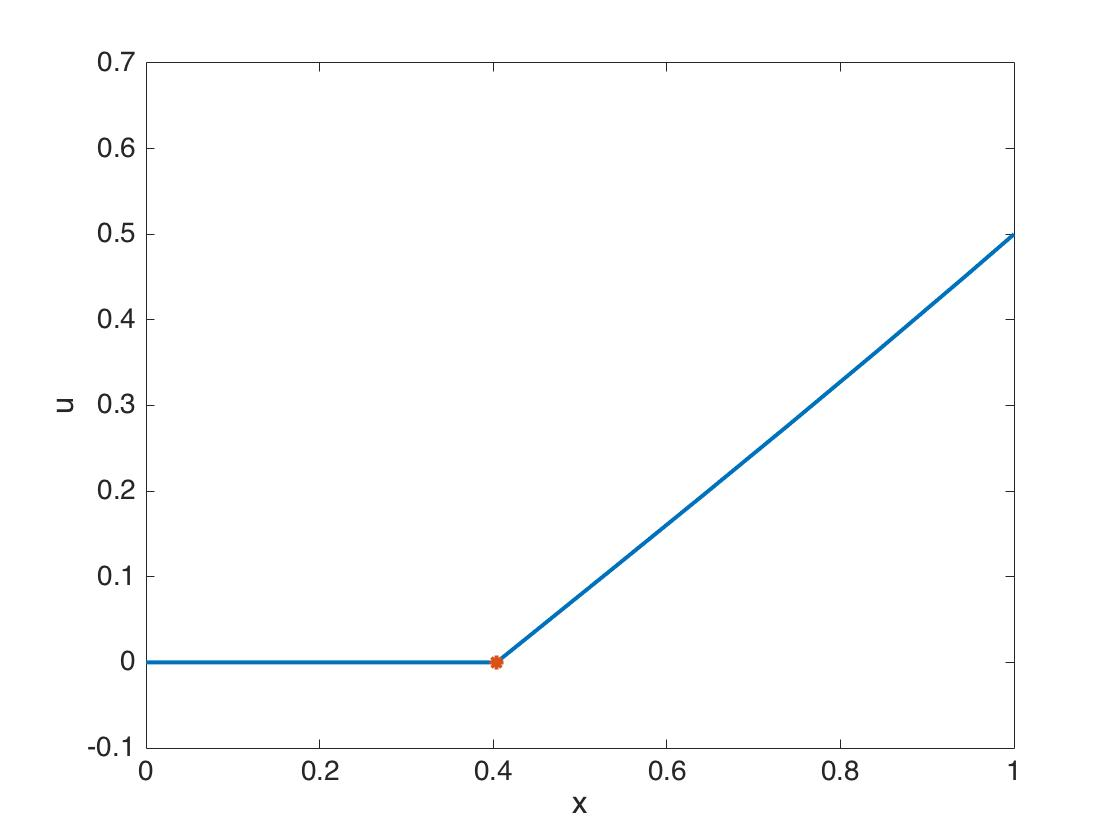
\includegraphics[width=3in]{sol1.jpg} 
   \caption{Example 1: Minimizer found using control Hamiltonian for relaxed problem in Example 1}
   \label{fig:sol1}
\end{figure}



{\bf Young's measure result:} We now relate the semi-analytic results to the optimal parametrized measure of the generalized problem,
\[ \tilde{I}[\mu] = \int_0^1 \int_\R (\xi^2-1)^2_* \;d\mu_x(\xi)+ u^2 \; dx \hspace{2cm} u(0) = 0 \;u(1) = 1/2\]

From Theorem \ref{t:pedregal}, we know that given a solution, $\bar{u}$, to the relaxed problem,  the optimal parametrized measure, $\mu$, satisfies $\overline{W}(u_x) = \int W(\xi) \;d\mu(\xi)$. Therefore, for this example the optimal measure is given by 
 \[ \mu_x = \left \{ \begin{array}{c c c}
\infty &\mbox{for} & u_x(x)< 0\\
\lambda \delta_0 + (1- \lambda) \delta_{a} & \mbox{for} & 0\leq u_x(x) < a\\
\delta_{u_x(x)} & \mbox{for} & a\leq u_x(x) 
\end{array} \right.
\]
where $a= \sqrt{2/3}$ and $\lambda = \dfrac{a-u_x(x)}{a}$.

In addition, the optimal parametrized measure satisfies $\bar{u}_x = \int \xi \;d\mu(\xi)$. Since the derivative of $\overline{u}(x)$ is zero on the interval $x \in [0,0.4039)$, for these values of $x$ the measure $\mu_x = \delta_0$. On the other hand, on the interval $x \in [0.4039,1]$ the derivative satisfies $\overline{u}_x(x)> \sqrt{2/3}$ so that for these values of $x$ the measure $\mu_x = \delta_{\bar{u}_x}$. Since the optimal parametrize measure, $\mu$, consists of single Dirac measures, the solution to the relaxed problem, $\overline{u}$, is also a classical solution to the original problem $I[u]$.


%%%%%%%%%%%%%%%%%%%%%EXAMPLE 2 %%%%%%%%%%%%%%%%%%%%%%%

{\bf \large Example 2:} 

Consider the fully nonconvex Bolza problem,
\[ I[u] = \int_{-1}^1 (u_x-1)^2 + (u^2-1)^2\;dx \hspace{2cm} u(-1) =0,\; u(1) =0.\]
and its relaxation,
\[ \bar{I}[u] = \int_{-1}^1 (u_x^2-1)^2_+ + (u^2-1)^2\;dx \hspace{2cm} u(-1) = 0, u(1) =0\]
where we now define
\[ (v^2-1)^2_+= \left \{ \begin{array}{c c c}
0 & \mbox{for} & |v|<1\\[2ex]
(v^2-1)^2 & \mbox{for} & |v| \geq1
\end{array} \right.
\]
{\bf Semi-analytic solution:} Since the relaxed functional is not convex in $u$, we do not expect to find unique minimizers. Still, we can write down the control Hamiltonian 
\[ H(u,v,p) = pv - (v^2-1)^2_+ - (u^2-1)^2\]
and use Theorem \ref{t:controlH} to find the necessary conditions that lead to solutions:
\[ \dot{u} = v \quad \dot{p} = (u^2-1)^2\]
\[ \frac{\partial H}{\partial v} = p - \partial(v^2-1)^2_+ =0 \qquad \frac{\partial^2 H}{\partial v^2} = -\partial^2(v^2-1)^2_+ \leq 0.\]
As in the previous example the last condition is always satisfied, while the requirement $\frac{\partial H}{\partial v} =0$ gives a formula for the costate function, $p$, in terms of $v$. This allows us to write the Hamiltonian in terms of $u$ and $v$,
\[ H(u,v,p(v) ) = \left \{\begin{array}{c c c}
 -(u^2-1)^2 & \mbox{for} & |v| <1\\
 (v^2-1)(3v^2+1) - (u^2-1)^2 & \mbox{for} & |v| \geq 1.
 \end{array} \right.
 \]

There are two cases depending on the value of $v$ at the point $x =-1$.  If initially we assume that $|v(-1)|<1$, then the Hamiltonian 
$$H(u(-1),v(-1),p(v(-1))) = -(u(-1)^2-1)^2=-1.$$ Because the Hamiltonian is a conserved quantity, to stay on the level set $H=-1$ we need $v\equiv 0$. This corresponds to the trivial solution $u \equiv 0$ which has energy $\bar{I}[0] = 4$. 

If on the other hand $|v(-1)|\geq 1$ then $\dot{p} = (12v^2-4) \dot{v} = 4u(u^2-1) $, leading to the following dynamical system,
\[ \dot{u} = v, \quad \dot{v} = \frac{u(u^2-1)}{3v^2-1}.\]
Notice that this is a reversible system, so that if $(u(x),v(x))$ is a solution, then so is $u(-x),-v(-x))$. 

Here again we have two options, $v > \pm 1$. In the case when $\dot{u} = v(-1)>1$ the function $u(x)$ must be initially increasing. So, there is a point $x^*$ where $u(x^*) =1$ and therefore $\dot{v}(x^*)=0$. 

To find the location of $x^*$ we notice that because the value $|v|\geq 1$, the derivative $\dot{u} \geq 1$. Integrating $\dot{u}$ from $x=-1$ to $x=x^*$ shows that $x^*$ is less than zero. Since the dynamical system is reversible, the solution is even with respect to the $x-$axis. This implies that the solution must satisfy $u=1$ and $v=0$ on the interval $(x^*,0]$ and that for values of $x \in (0,1]$ the solution must mirror what happens in the interval $[-1,0)$, allowing $u$ to satisfy the boundary at $x=1$. In addition, since $u=1$ and $v=0$ on $(x^*,-x^*)$ the solution must lie on the level set $H=0$ and because we jump to values of $|v|\geq 1$, at $x=x^*$ we must have that $v(x^*) = 1$.

 To find the value of $x^*<0$ and the solution on the interval $[-x^*,1]$ we can integrate the above equations using as initial conditions $u(0)=1$ and $v(0)=1$ and stoping as soon as $u(1+x^*)=0$. With this process we find numerically that $x^* = 0.0529$. 
 
 If we denote  the solution to the dynamical system by $u^*$, we can say that the solution, $\bar{u}$, to the relaxed functional is given by,
\begin{equation}\label{e:sol}
[ \overline{u}(x)  = \left \{ \begin{array}{c c c}
u^*(-x) & \mbox{for} & -1\leq x \leq x^*\\
1 & \mbox{for} & x^*< x< -x^*\\
u^*(x) & \mbox{for} & -x^*\leq x \leq1
\end{array} \right. \tag{*'}
\end{equation}
where $x^*=0.0529$ and $u^*$ satisfies $|u^*_x|\geq 1 $. A plot of $u^*(x)$ is shown in Figure \ref{fig:sol3}. The numerical approximation for these solutions found in the next section shows that their energy, $I[u] = 1.2787$, is much smaller than that of the trivial solution $u=0$, which we saw has energy $I[0] = 4$. 

\begin{figure}[htbp] %  figure placement: here, top, bottom, or page
   \centering
   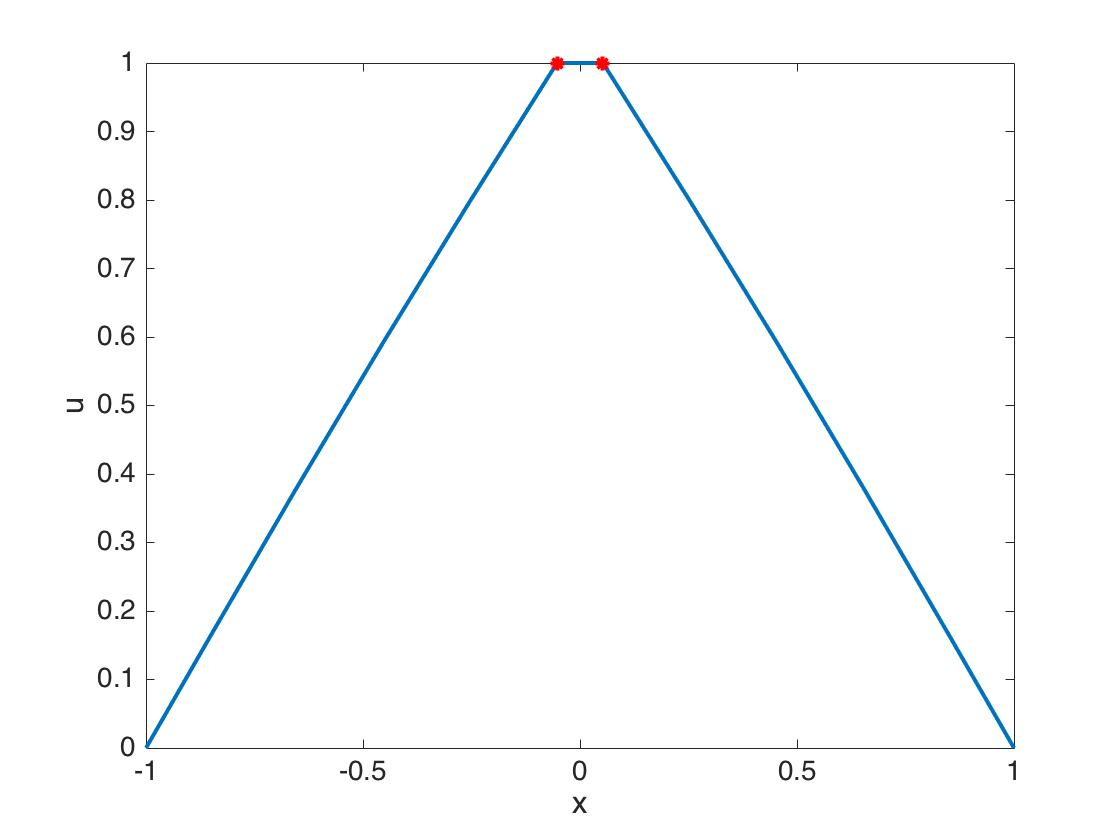
\includegraphics[width=3in]{sol3.jpg} 
   \caption{Minimizer found using control Hamiltonian for relaxed problem in Example 3}
   \label{fig:sol3}
\end{figure}
For the second case when $v<-1$, the argument is very similar as the one presented above. The solution in this case is just $-u^*(x)$.

{\bf Young's measure:} We now continue by relating the semi-analytic result given by \eqref{e:sol} to the generalized functional,
\[ \tilde{I}[\mu] = \int_{-1}^1 \int_\R (\xi -1)^2 \;d\mu_x(\xi) + (u^2-1)^2\;dx \quad u(-1) =0,\; u(1) =0.\]
We know that the optimal parametrized measure, $\mu$, must satisfy $\overline{W}(u_x) = \int W(\xi) \;d\mu(\xi)$ leading to
\[ \mu_x = \left \{ \begin{array}{c c c}
\lambda \delta_{-1}+ (1-\lambda) \delta_{1} & \mbox{if} & |u_x| < 1\\
\delta_{u_x} & \mbox{if} & |u_x|\geq 1
\end{array} \right. \]
where $\lambda = \frac{ 1- u_x}{2}$. Since the optimal measure must also satisfy  $\bar{u}_x = \int \xi \;d\mu(\xi)$, we look at the solution to the relaxed problem we found above.

First notice that for all $ x\in [-1,x^*] \cup [-x^*,1]$ the derivative $|\bar{u}'(x)| >1$, implying that  $\mu= \delta_{\bar{u}'}$ on these intervals. On the other hand, for $ x\in (x^*,-x^*)$ we have that $\bar{u}'(x) =0$ and as a result $\mu = \frac{1}{2} \delta_{-1} + \frac{1}{2} \delta_{1}$ and we may conclude that minimizing sequences exhibit oscillations on this interval. To find the scale of this oscillations we consider the regularized problem 
\[ I^\eps[u] = \int_{-1}^1 \eps^2 u_{xx}^2 + (u_x^2-1)^2 + (u^2-1)^2\;dx \quad u(-1) = 0 \; u(1) = 0\]
A scaling argument then suggests that given any $\eps>0$ these oscillations will have wavelengths of order $\lambda \sim \eps^{1/5}$. 



 
 
%%%%%%%%%%%%%%%%%%%%%%%%%%%%%%%%%%%%%%%%%%%%%%%%%%%%%%%%%%%%%%%%
%%%%%%%%%%%%%%%%%%%%%%%% SPLIT BREGMAN %%%%%%%%%%%%%%%%%%%%%%%%%%%%%%

\section{Computing the relaxation numerically}\label{s:computations}
In this section, we propose a numerical scheme for finding minimizers of nonconvex problems as defined in the introduction. For convenience we reformulate them here in a more compact form,
\begin{equation}\label{e:relaxed}
 \min_{u}  \overline{W}[u_x] + V[u] \qquad u-u_0 \in W^{1,p}_0(\Omega),
 \end{equation}
where  $\overline{W}[d] = \int_\Omega \overline{W}(d)$ and we use a similar notation for $V[u]$. 

To numerically compute these minimizers we use a two step process. First, we numerically compute the convex envelope of the nonconvex integrand $W(d)$ by recasting the problem as an obstacle problem. This can be done using the method presented in Tran et al. \cite{tran2015}, where the Split Bregman algorithm is adapted to solve this type of problems. The result of this process is a piecewise linear function that plays a similar role to the $L^1$ norm, a nice fact that will allow us to use a modified shrink operator as part of our algorithm. This will also allow us to treat cases where there is no analytic description of this convex envelop. 

The second step is to pose the problem as a gradient flow problem and look for steady solutions of  $u_t = -\dfrac{\delta \overline{I}}{\delta u}$, keeping in mind that these solutions correspond to local minima. This means that in order to find a minimizer of $\bar{I}$ we also have to compare all steady states and choose the solution that corresponds to the absolute minimum of $\bar{I}$. This does present a problem, mainly how do we know that we have found a global minimum. Nonetheless, the approach is still powerful since it allows us to consider the case when $V[u]$ is also a nonconvex functional by incorporating a convex splitting scheme into our algorithm. 
 
We emphasize again that the goal is to use the solutions of the relaxed problem to infer existence of classical minimizers for the original problem $I$, or in the case when these minimizers do not exist, use scaling arguments derived from the regularization, ~\eqref{e:regularized}, to find the length scale of oscillations in minimizing sequences. At the end of this section we will consider again the examples from Section \ref{s:controlH} and compare them to the numerical results found using our algorithm.


 As a start we present a modified version of the Split Bregman algorithm, which we use here for finding minimizers of problems of the form \eqref{e:relaxed} where both $\overline{W}[d]$ and $V[u]$ are convex functionals. The power of this scheme is that it allows us to decouple the these two terms through the constraint, $d= u_x$ and write the the problem in an equivalent formulation,
\begin{equation}\label{e:constrain}
 \min_{u,d}  \overline{W}[d] + V[u] \quad \mbox{subject to} \quad u_x = d.
 \end{equation}
 Recasting it as an unconstrained problem 
\[ \min_{u,d}   \overline{W}(d) + V[u] + \frac{\lambda}{2} \| u_x - d\|^2,\]
 minimizers are sought by iterating the following scheme,
\begin{align*}
(u^{k+1},d^{k+1}) =& \mbox{argmin}_{u,d} \overline{W}[d] + V[u] + \frac{\lambda}{2} \| u_x - d -b^k\|^2\\
b^{k+1} = & b^k - (u_x^{k+1} - d^{k+1}).
\end{align*}
In addition, because the functionals $\overline{W}$ and $V$ are now decoupled, one can solve the minimization in two steps,
\begin{align*}
u^{k+1}  =& \mbox{argmin}_{u,d}  V[u] + \frac{\lambda}{2} \| u_x - d^k, -b^k\|^2\\
d^{k+1} =& \mbox{argmin}_{u,d} \overline{W}[d] + \frac{\lambda}{2} \| u_x^{k+1} - d -b^k\|^2.
\end{align*}
The first subproblem can solved using for example a conjugate gradient method or Gauss-Seidel, while the second can be solved by a piecewise linear shrink operator, which we define in \eqref{e:shrink}.

  The main advantage of this algorithm is that is easy to implement and fast to converge. In addition, and as opposed to other constraint optimization methods,  the constraint parameter $\lambda$ is fixed and can be chosen to minimize the condition number of the subproblems. These subproblems also don't need to be solved to full accuracy since the Split Bregman iteration has a built in error forgetting property \cite{yin2013}. More importantly, fixed points of the Bregman iteration are solutions to the constraint problem ~\eqref{e:constrain}. This last result is important and a proof based on the results from  \cite{osher2005} and adapted to our present problem can be found in the Appendix \ref{s:appendixB}.


Notice that as it is written now, we are not able to use the algorithm to find minimizers of functionals with $V[u]$ nonconvex. This is because the Euler Lagrange equations that result from the first subproblem are ill posed.  We could instead recast the problem as a gradient flow problem combined with a convex splitting method.  The difficulty then is that because our convex envelope $\overline{W}$ is not continuously differentiable, the evolution equation contains nonsmooth coefficients. Instead, the approach we take here is to combine these two methods, the convex splitting scheme together with the Modified Split Bregman algorithm. To describe the method we first review the main ideas behind convex splitting schemes.


As the name suggest, these numerical algorithms consists in splitting a nonconvex functional, $\bar{I}$, into a convex part, $\bar{I}_+$, and a concave part, $\bar{I}_-$. Then using the weak formulation the gradient equation is written as,
\[ \langle u_t,w \rangle  = - ( \frac{\delta \bar{I}+}{\delta u}[u],w) -( \frac{\delta \bar{I}-}{\delta u}[u],w).   \]
where $u \in u_0 + H^1_0(\Omega)$ and $\langle \cdot, \cdot\rangle$ is the inner product in $H^1_0(\Omega)$. Since the nonconvex part leads to ill posed equations, this term is evaluated at a previous time step and treated as a forcing term. For a time step of $h$, the algorithm then consist in solving,
\[ \langle \frac{u_{n+1}-u_n}{2h}, w \rangle  = \left(  \frac{\delta \bar{I}+}{\delta u}[u_{n+1}],w \right) - \left ( \frac{\delta \bar{I}-}{\delta u}[u_n],w \right).\]

The key idea is to realize that this equation is formally the Euler Lagrange equation for the Rayleigh functional
\[ R^n[v] = \frac{1}{2h}\langle v-u_n, v - u_n \rangle + \bar{I}_+[v] + \left ( \frac{\delta \bar{I}-}{\delta u}[u_n],v-u_n \right) + \bar{I}_-[u_n] \]
where the last two terms are the linearization of $\bar{I}_-$ at $u_n$. 

Our numerical scheme seeks to find minimizers of the Rayleigh functional using the Modified Split Bregman algorithm described above. This is possible since this functional is strictly convex, so that minimizers exist and are unique. Moreover, as shown in \cite{glasner2016}, the sequence of iterates $\{u_n\}$ converges to local minima of $\bar{I}$, so that process converges to the right solution. For completeness we restate this last result in the following lemma and provide a short proof.

\begin{Lemma}\label{l:localmin}
The sequence $\{u_n\}$ generated by minimizing the Rayleigh functional at each time step converges to local minima of $\bar{I}$.
\end{Lemma}
\begin{proof}
We first show that the algorithm is energetically stable, that is we show that each iterate decreases the energy. Suppose that $u_{n+1}$ is a minimizer for $R^n[v]$, then it is straight forward to show that $$\bar{I}[u_{n+1}] \leq R^n[u_{n+1}] \leq R^n[u_n] = \bar{I}[u_n].$$
The first inequality follows from the definition of $R^n$ and the fact that the linearization of the concave part $I_-$ about $u_n$ lies above this functional. The second inequality says that $u_{n+1}$ is the minimizer for $R^n$, and the last equality follows from the definition of $R^n$.

Since $\bar{I}[u_n]$ is a decreasing sequence bounded from below, it converges to a local minimum, $\bar{m}_l$. Because the functional $\bar{I}$ is coercive and lower semicontinuous, the sequence of iterates $\{u_n\}$ converges weakly to a function $\bar{u}$ with $\bar{I}[\bar{u}] = \bar{m}_l$.
\end{proof}

Our proposed algorithm which minimizes the Rayleigh functional $R^n$ using the Modified Split Bregman algorithm is given next.

\begin{framed}
{\Large \texttt Algorithm}

Given $ tol_1$ and parameters $\lambda,h$


set $u^0=0$ and $b^0=0$



{\bf While} $\|u^k - u^{k+1}\|_2 > tol_1$ {\bf do}
\begin{align*}
(u^{k+1},d^{k+1}) =& \;\mbox{argmin}_{(u,d)}\quad \frac{1}{2h} \|u-u^k\|_2^2 + \overline{W}[d] +V_+[u]+(\delta V_-[u^k],u-u^k) + V_-[u^k] \\[2ex]
&\hspace{10ex}+ \frac{\lambda}{2} \|u_x-d-b^k\|_2^2\\[2ex]
b^{k+1} =&\; b^k - (u_x^{k+1}-d^{k+1})
\end{align*}



{\bf end}
\end{framed}


%\begin{framed}
%{\Large \texttt Algorithm}
%
%Given $U_0, tol_1,tol2$ and parameters $\lambda,h$
%
%
%
%{\bf While} $\|U_n - U_{n+1}\|_2> tol_1$ {\bf do}
%
%set $u_0=0$ and $b=0$
%
%{\bf While} $\|u^k - u^{k+1}\|_2 > tol_2$ {\bf do}
%\begin{align*}
%(u^{k+1},d^{k+1}) =& \;\mbox{argmin}_{(u,d)}\quad \frac{1}{2h} \|u-U_n\|_2^2 + \overline{W}[d] +V_+[u]+(\delta V_-[U_n],u-U_n) + V_-[U_n] \\[2ex]
%&\hspace{10ex}+ \frac{\lambda}{2} \|u_x-d-b^k\|_2^2\\[2ex]
%b^{k+1} =&\; b^k - (u_x^{k+1}-d^{k+1})
%\end{align*}
%{\bf end}
%
%$U_{n+1} = u^{k+1}$
%
%
%{\bf end}
%\end{framed}





As mentioned before, the minimization can be carried out as two step process.

\begin{align*}
u^{k+1} = &  \;\mbox{argmin}_{u}\quad \frac{1}{2h} \|u-u^k\|_2^2  +V_+[u]+(\delta V_-[u^k],u-u^k) + V_-[u^k] + \frac{\lambda}{2} \|u_x-d^k-b^k\|_2^2,\\[2ex]
d^{k+1} = & \;\mbox{argmin}_{d}\quad  \overline{W}[d] + + \frac{\lambda}{2} \|u^{k+1}_x-d-b^k\|_2^2.
\end{align*}
We solve the first problem by finding solutions to the corresponding Euler-Lagrange equations using Gauss-Seidel. To solve the second step we think of the gradient as piecewise linear function,
\[\partial \overline{W}(d) = s_i \quad \mbox{for}\quad d_{i-1}\leq d < d_i\]
where $d_i$ are points where $\partial\overline{W}$ is discontinuous. Then the minimization can be done using the piecewise shrink operator $S_p$, defined as follows:
\begin{equation}\label{e:shrink}
S_p\left (\frac{s_i}{\lambda},z\right) = \left \{ z- \frac{s_i}{\lambda} \quad \mbox{for} \quad d_{i-1}+\frac{s_i}{\lambda} \leq z < d_i+\frac{s_i}{\lambda} \right.
\end{equation}
with $z = u_x^{k+1}-b^k$.
Finally, we conclude with a review of the examples from Section \ref{s:controlH}.

{\bf Examples 1}
We numerically find minimizers of the functional
\[ \bar{I}[u] = \int_{-1}^1 (u_x^2-1)_+^2 + u^2 \;dx \quad u(0) = 0,\; u(1) = 0,\]
where $(d^2-1)^2_+$ represents the convex envelop of the piecewise function $(d^2-1)_*^2$, described in Section \ref{s:controlH}. In Figure \ref{f:example1} the numerical results are plotted against the analytic solutions found in Section \ref{s:controlH} showing that they are in good agreement.

\begin{figure}[h]
\centering
    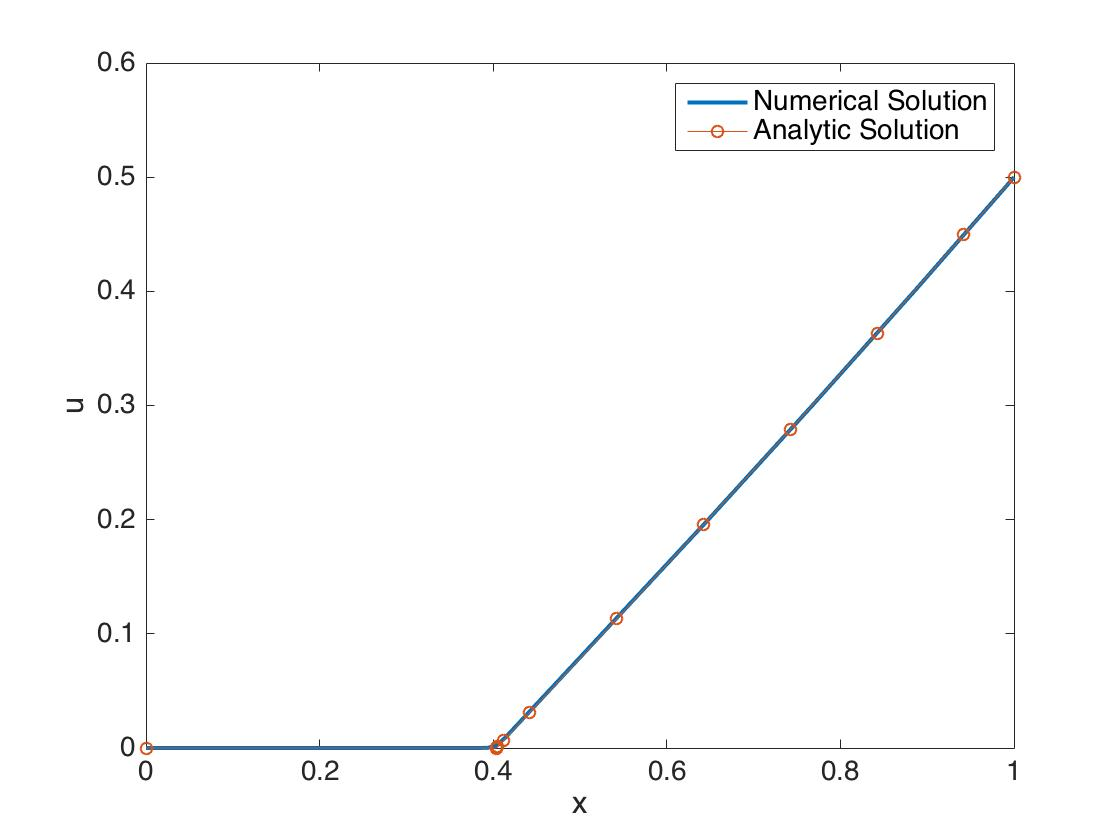
\includegraphics[width=0.4\textwidth]{Ex1NumSol.jpg}
 \caption{Numerical results for local minimizers of Example 1 using Modified Split Bregman together with Gradient Flow. This solution has an approximate energy of $I[u]0 = 0.5061$}\label{f:example1}
\end{figure}

{\bf Example 2}
Here we consider a functional which is nonconvex in the variable $u$. 
\[ \bar{I}[u] = \int_{-1}^1 (u_x^2-1)_+^2 + (u^2-1)^2 \;dx \quad u(-1) = 0,\; u(1) = 0.\]
In this example the function $(d^2-1)^2_+$ now represents the convex envelop of the polynomial $(d^2-1)^2$. In Figure \ref{f:example2}, we plot the two global minimizers agains their semi-analytic counterpart found in Section \ref{s:controlH}.


\begin{figure}[h]
\centering
\subfloat[]
{
    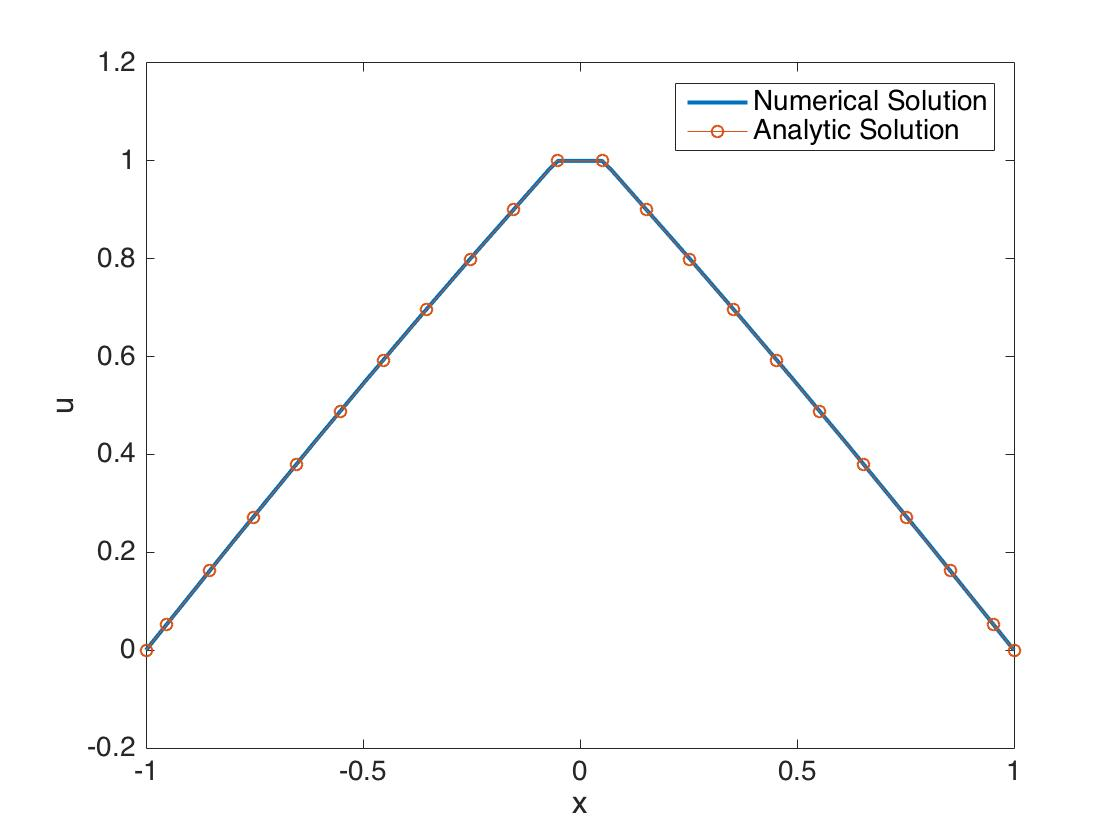
\includegraphics[width=0.4\textwidth]{GF-MSP.jpg}
%    \label{fig:fdsk}
}
\subfloat[]
{
    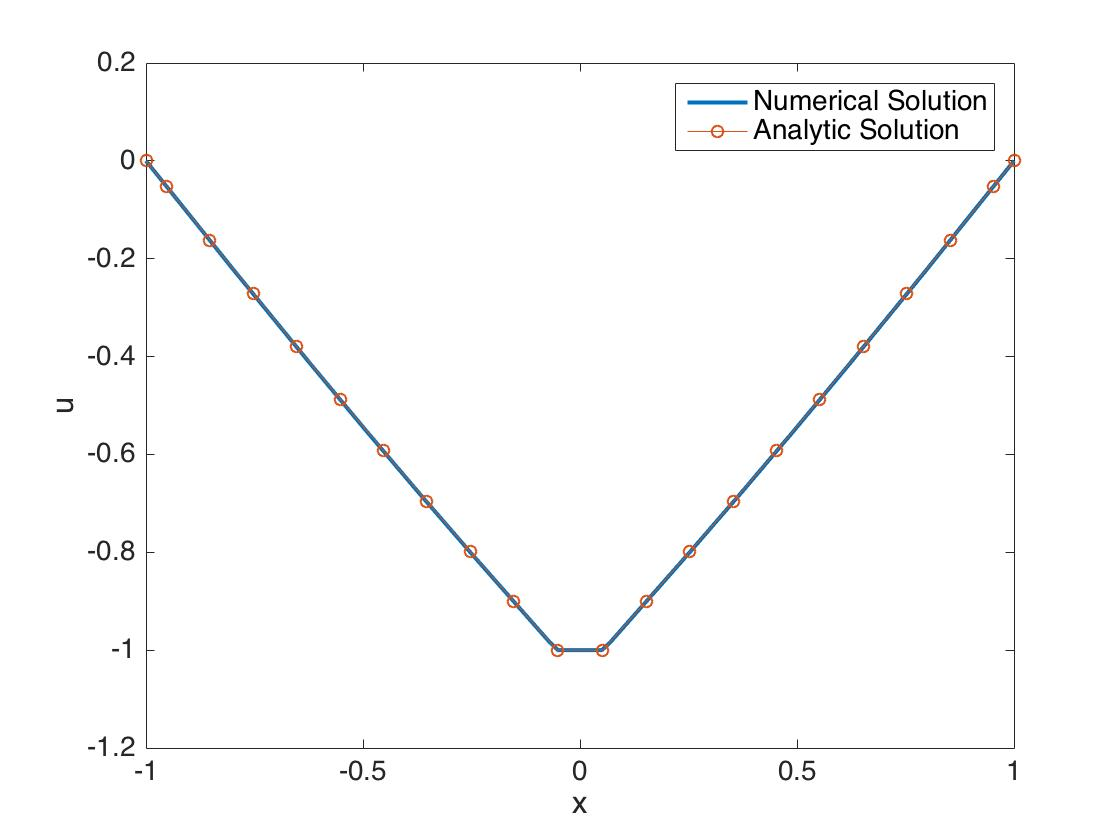
\includegraphics[width=0.4\textwidth]{GF-MSP-2.jpg}
 %   \label{fig:foo-2}
}
 \caption{Numerical results for local minimizers of Example 2 using Modified Split Bregman together with Gradient Flow. Figure a) corresponds to an initial guess of $u =1$ and figure b) corresponds to an initial guess of $u =-1$. Both solutions have an approximate energy of $I[u] = 1.1287$ }\label{f:example2}
\end{figure}


{\bf Example 3}:

We look at a variation of Example 2 with a triple well potential,
\[ \bar{I}[u] = \int_{-1}^1 [(u_x^2-1)( (u_x-2)^2 -1)^2]_+ + (u^2-1)^2 \;dx \quad u(-1) = 0,\; u(1) = 0.\]
where $[(u_x^2-1)( (u_x-2)^2 -1)^2]_+$ is the convex envelope of $(u_x^2-1)( (u_x-2)^2 -1)^2$. A plot of this function is given in Figure \ref{f:example3} together with a plot of the  minimizers of this functional. The Young measure $\mu$ which satisfies $\bar{u} = \int \xi \;d\mu(\xi)$ and $\overline{W}(\bar{u}_x = \int W(\xi) \;d\mu(\xi)$ is 
\[ \mu = \left\{ \begin{array}{c c c}
\delta_\xi & \mbox{for} & \xi < -1\\
\lambda \delta_{-1} + (1- \lambda) \delta_3 & \mbox{for} &-1\leq  \xi \leq 3\\
\delta_\xi & \mbox{for} & \xi < -1
\end{array} \right.
\]
with $\lambda = \dfrac{3 -\xi}{4}$ and $\xi$ plays the role of $\overline{u}_x$.

\begin{figure}[h]
\centering
\subfloat[]
{
    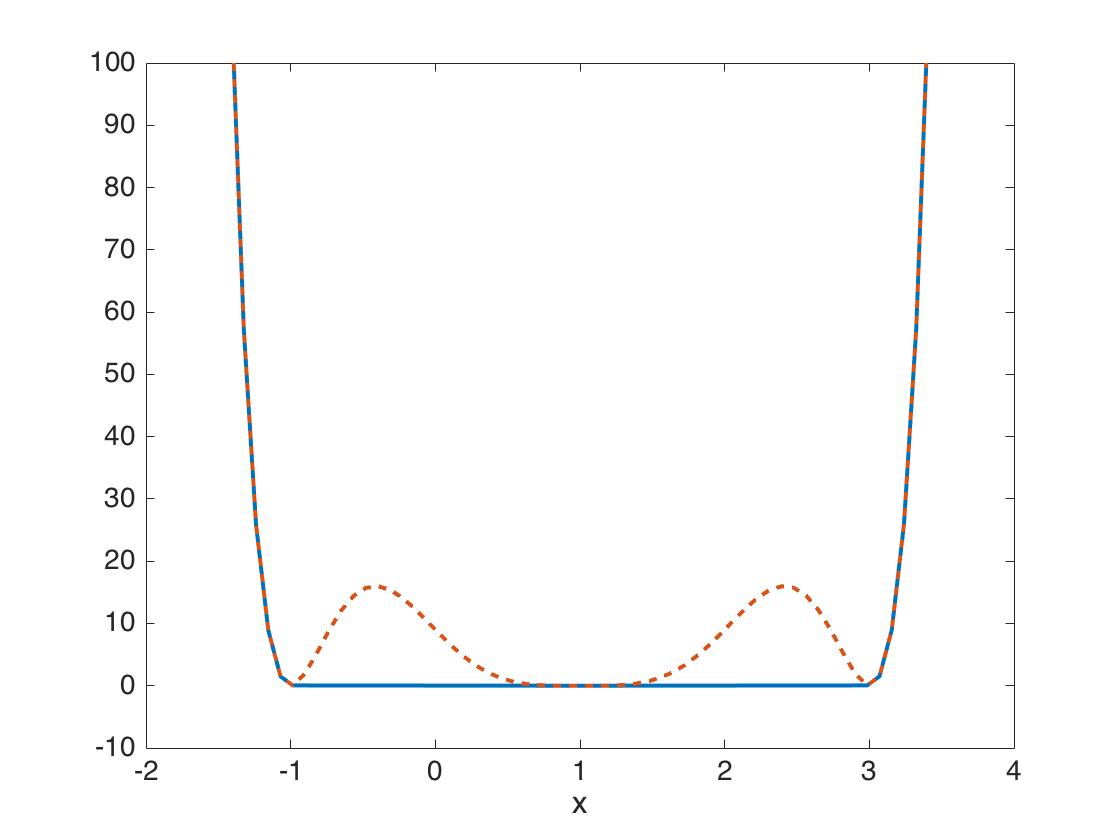
\includegraphics[width=0.4\textwidth]{ConvexEnv.jpg}
%    \label{fig:fdsk}
}
\subfloat[]
{
    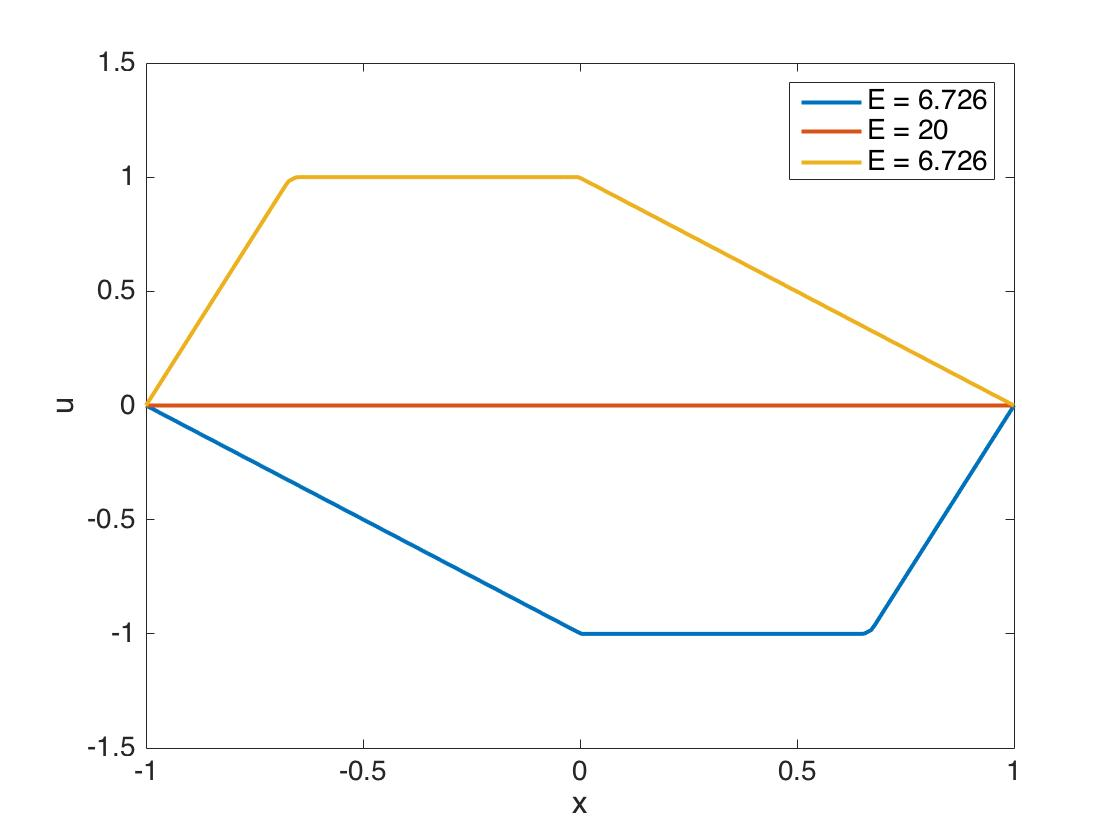
\includegraphics[width=0.4\textwidth]{Ex3NumSol.jpg}
 %   \label{fig:foo-2}
}
 \caption{a) Convex envelop for $W(d)= (d^2-1)^2( (d-2)^2-1)^2$. b) The three minimizers for the relaxed energy $\overline{I}[u]$ in  Example 3
 }\label{f:example3}
\end{figure}

It is clear from Figure \ref{f:example3} that there are two global minimizers for this problem, both with energy $\bar{I}[u]=6.106$. If we now consider the gradient of these solutions, see Figure \ref{f:gradientE3}, we are able to find the optimal measure for the generalized problem $\tilde{I}[\nu]$. Labeling the two minimizers of the relaxation as $u_+$ and $u_-$ for the positive and negative solutions, respectively, then their associated Young measures, $\mu_+, \mu_-$ are
\begin{figure}[h]
\centering
\subfloat[]
{
    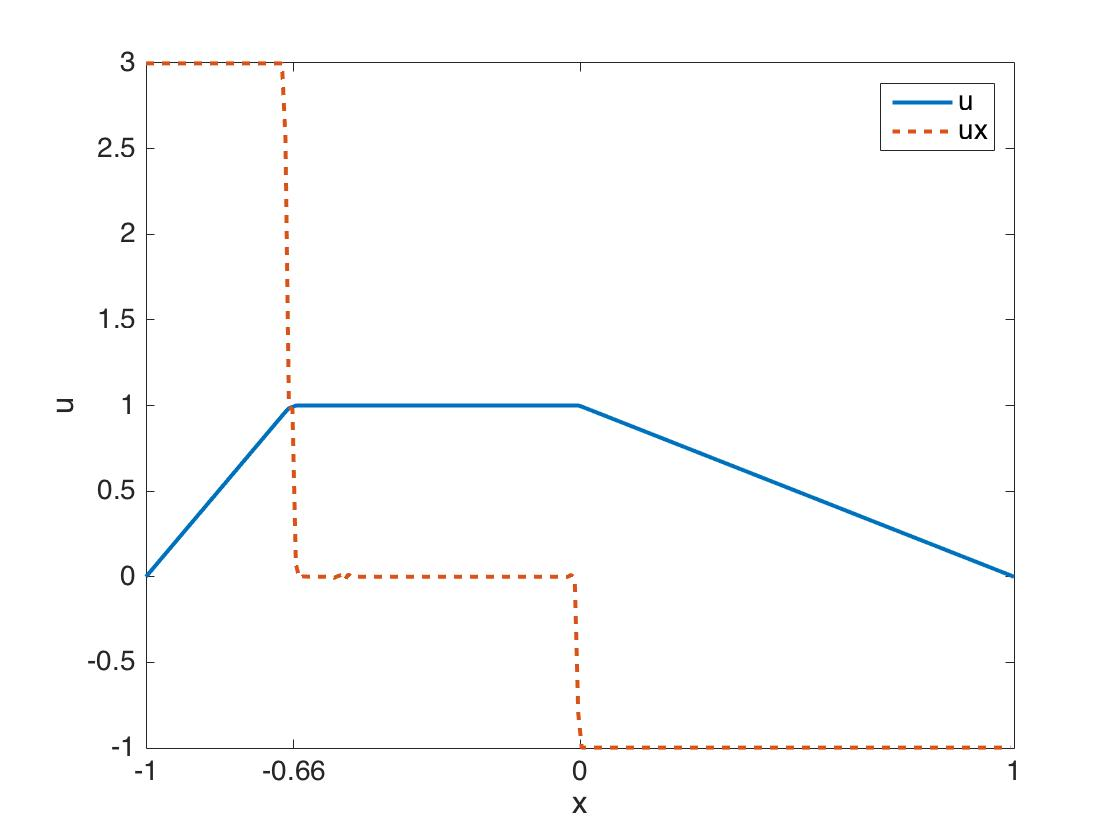
\includegraphics[width=0.4\textwidth]{gradientplus.jpg}
%    \label{fig:fdsk}
}
\subfloat[]
{
    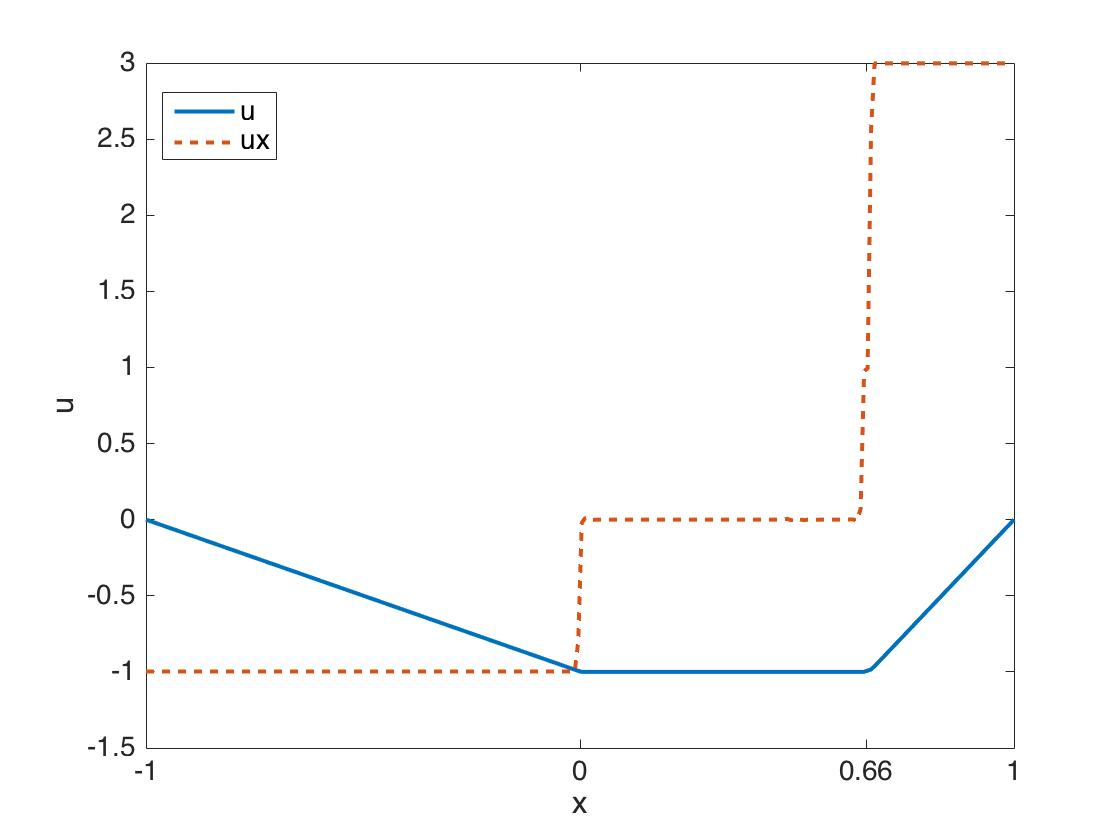
\includegraphics[width=0.4\textwidth]{gradientneg.jpg}
 %   \label{fig:foo-2}
}
 \caption{Minimizers and their gradients
 }\label{f:gradientE3}
\end{figure}

\[ \mu_+ = \left \{ 
\begin{array}{c c c}
\delta_3 & \mbox{for}& -1\leq x\leq -0.66\\
\frac{3}{4} \delta_{-1} + \frac{1}{4}\delta_3 & \mbox{for} & -0.66< x < 0\\
\delta_{-1} & \mbox{for} & 0 \leq x \leq 1
\end{array} \right.
\qquad 
\mu_- = \left \{ 
\begin{array}{c c c}
\delta_{-1} & \mbox{for}& -1\leq x\leq 0\\
\frac{3}{4} \delta_{-1} + \frac{1}{4}\delta_3 & \mbox{for} & 0< x < 0.66\\
\delta_{3} & \mbox{for} & 0.66 \leq x \leq 1
\end{array} 
\right.
 \]


%%%%%%%%%%%%%%%%%%%%%%%%%%%%%%%%%%%%%%%%%%%%%%%%%%%%%%%%%%%%%%%%
%%%%%%%%%%%%%%%%%%%%%%%% APPENDIX A%%%%%%%%%%%%%%%%%%%%%%%%%%%%%%

\section{Appendix A}\label{s:AppendixAA}

In this section we give a sketch of the proof of Proposition \ref{p:GammaLimit}, which we rewrite here for convenience. 

\begin{Proposition*}
Let $X$ be a Banach space whose dual $X^*$ is a separable space, and let  $\{F_n: X \rightarrow \overline{R}\}$ be a family of functionals that is bounded bellow by $\Psi: X \rightarrow \overline{R}$, such that
\[ \lim_{\|x\|_X \rightarrow \infty } \Psi(x) = + \infty.\]
 Assume as well that this family is a decreasing sequence converging pointwise to $F:X \rightarrow \overline{R}$, then the sequence $\Gamma-$converges to the lower semicontinuous envelope of $F$, $sc^-F$.
\end{Proposition*}


The proof relies on the following definition of the $\Gamma$ limit and Propositions 5.7 and 8.10 from \cite{dal2012introduction}. Here $\mathcal{N}(x)$ represents the set of all open neighborhoods of $x$.

\begin{Definition}[Dal Maso, Definition 4.1]\label{d:gamma}

We define  the $\Gamma$ lower and upper limits of the sequence $F_n:X \rightarrow \overline{\R}$ are as
\begin{align*}
(\Gamma-\liminf_{n \to \infty} F_n)(x) &= \sup_{U \in \mathcal{N}(x)} \liminf_{n \to \infty} \inf_{y \in U} F_n(y)\\
(\Gamma-\limsup_{n \to \infty} F_n)(x) &= \sup_{U \in \mathcal{N}(x)} \limsup_{n \to \infty} \inf_{y \in U} F_n(y).
\end{align*}

Moreover, if there is a function $F:X\rightarrow \overline{R}$ such that $\Gamma-\liminf_{n \to \infty} F_n= \Gamma-\limsup_{n \to \infty} F_n$ then we write 
\[ F = \Gamma-\lim_{n \to \infty} F_n\]
and we say that the sequence, $F_n$, $\Gamma$- converges to $F$ in X.

\end{Definition}

Using this definition one is able to show that
\begin{Proposition*}[Dal Maso, Proposition 5.7]
If $F_n$ is a decreasing sequence converging pointwise to $F$ then the sequence, $F_n$, $\Gamma$ converges to the lower semicontinuous envelope of $F$, $sc^-F$.
\end{Proposition*}

Proposition 5.7 uses the above definition of $\Gamma$ convergence, which relies on the topology of $X$.  In order to proof  Proposition \ref{p:GammaLimit} we need to establish the equivalence between Definition \ref{d:gamma} and $\Gamma$ convergence in terms of sequences. This is possible if we endow $X$ with a topology that has the first axiom of countability, as stated in Proposition 8.1 in \cite{dal2012introduction}). However, in our case and in general applications one usually works with the weak topology of $X$, which does not provide a countable neighborhood basis for every point. This means that in order to establish the equivalence  we need to impose extra conditions. In particular, if the dual space, $X^*$, is separable and the sequence $F_n$ is bounded from below by a coercive function,  Proposition 8.10 in \cite{dal2012introduction}) shows that both definitions of $\Gamma$ convergence coincide. Before sumarizing Proposition 8.10 we will need the following definitions.

Here we consider $d$ to be the metric on $X$ induced by a dense sequence $f_n$ in the unit ball of $ X^*$, so that for any $x,y \in X$
\[ d(x,y) = \sum_n \frac{1}{2^n} \left | \langle f_n, x-y, \rangle \right|\]
where $\langle \cdot, \cdot \rangle$ represents the pairing between elements in $X$ and its dual. 
We also define 
\begin{align*}
 F' (x) = (\Gamma-\liminf_{n \to \infty} F_n)(x) & \qquad F'' (x) = (\Gamma-\limsup_{n \to \infty} F_n)(x) \\
 F_d' (x) = (\Gamma-\liminf_{n \to \infty} F_n)(x) & \qquad F_d'' (x) = (\Gamma-\limsup_{n \to \infty} F_n)(x) 
\end{align*}


With the above notation we are ready to restate Propositon 8.10 from \cite{dal2012introduction})
\begin{Proposition*}[Dal Maso, 8.10]
Assume $X$ is a Banach space endowed with its weak topology and that its dual $X^*$ is separable. Let $\Psi : X \rightarrow \overline{R}$ be such that
\[ \lim_{\| x\| \to \infty} \Psi(x) = +\infty\]
and assume $F_n \geq \Psi$ for every $n \in \N$. Then
\begin{enumerate}
\item $F' = F'_d$ \quad $F''= F''_d$
\item For every $x \in X$ and every sequence $\{x_n\}$ converging weakly to $x$ in $X$ we have
\[ F'(x) \leq \liminf_{n \to \infty} F_n(x_n)\]
\item For every $x \in X$ there is a sequence $\{x_n\}$ converging weakly to $x$ in $X$ such that
\[ F'(x) = \liminf_{n \to \infty} F_n(x_n)\]
\item For every $x \in X$ and every sequence $\{x_n\}$ converging weakly to $x$ in $X$ we have
\[ F'(x) \leq \limsup_{n \to \infty} F_n(x_n)\]
\item For every $x \in X$ there is a sequence $\{x_n\}$ converging weakly to $x$ in $X$ such that
\[ F'(x) = \limsup_{n \to \infty} F_n(x_n)\]
\end{enumerate}
Therefore $F_n$ $\Gamma$ converges to $F$ if and only if the following conditions are satisfied.
\begin{enumerate}
\item  For every $x \in X$ and every sequence $\{x_n\}$ converging weakly to $x$ in $X$ we have
\[ F'(x) \leq \liminf_{n \to \infty} F_n(x_n)\]
\item For every $x \in X$ there is a sequence $\{x_n\}$ converging weakly to $x$ in $X$ such that
\[ F'(x) = \limsup_{n \to \infty} F_n(x_n)\]
\end{enumerate}
\end{Proposition*}





%%%%%%%%%%%%%%%%%%%%%%%%%%%%%%%%%%%%%%%%%%%%%%%%%%%%%%%%%%%%%%%%
%%%%%%%%%%%%%%%%%%%%%%%% APPENDIX B%%%%%%%%%%%%%%%%%%%%%%%%%%%%%%

%\section{Appendix B}\label{s:appendixA}
%
%The approach we take here is to treat the problem of finding the convexification of a smooth function $W:\Omega \rightarrow \R $, where $\Omega \subset \R$ is bounded, as an obstacle problem. That is, we want to find the function $u$ that minimizes the Dirichlet energy 
%\begin{equation}\label{e:obstacle}
% J[u] = \frac{1}{2} \int_\Omega | \nabla u|^2 
% \end{equation}
%and lies above the obstacle $ \phi(x) = -W(x) + \alpha$, where $\alpha = \max_\Omega W(x)$. Then the convex envelop is given by $\bar{W}(x) = -u(x)+\alpha$. How do people solve this problem but not using L1 regularization?
%
%We use here the algorithm proposed by Tran et al. \ref{tran2015penalty}, where the associated unconstrained problem is solved: Minimize the energy
%\begin{equation}\label{e:o-unconstrained}
% J_\mu(u) = \int_\Omega \frac{1}{2} |\nabla u |^2 + \mu( \phi - u)_+
% \end{equation}
%where in this context $\mu( \phi - u)_+ = \max \{ \phi -u, 0\}$, and the minimization is done over all functions $u \in H^1_0$.
%
%It has been shown \cite{friedlander2008regularization, magasarian1985sufficiency} that if $\mu$ is large enough then both problems, \eqref{e:obstacle} and \eqref{e:o-unconstrained}, are equivalent. That is, if $u$ and $u_\mu$ are a minimizer for the Dirchlet energy and the unconstrained problem respectively, then provided $\mu$ is large enough $u = u_\mu$. In \cite{tran2015penalty} the authors give a lower bound for the constrained parameter $\mu$, requiring $\mu \geq -\Delta \phi$, where $\phi$ represents the obstacle. For us this means $\mu \geq  \Delta W$. If this condition holds then one is able to proof that given any $v \in H^1_0$, the function $ v + ( \phi- v)_+$ has lower $J_\mu$ energy than $v$. Moroever, if $u_\mu$ is the unique minimizer for $J_\mu$ then we must have $(\phi - u_\mu)_+ =0$. In other words $u_\mu \geq \phi$, which shows that this function is an admissible function for the orginal Dirichlet problem, $J$. Because $(\phi - u_\mu)_+ =0$, this also implies that $J_\mu(u_\mu) = J(u_\mu)$ showing that
%\[ J(u_\mu) = J_\mu(u_\mu) \leq J_\mu(u) = J(u)\]
%for any other $u$ in the admissible set of $J$. Therefore $u_\mu$ is also a minimizer for the original problem $J$, and the unconstrained problem results in an exact penalty if $\mu \geq -\Delta \phi$.??
%
%{\bf Algorithm}
%The obstacle problem \eqref{e:o-unconstrained} consists in minimizing a convex energy that depends on the gradient, subject to a constrain. The constrain can be enforced as an $\ell^1$ penalty and minimizers for this new energy can be found using the Split Bregman algorithm \cite{goldstein2009}. Introducing the variable $v = \phi -u$ the algorithm can be written as
%\begin{align*}
%(u^{k+1}, v^{k+1}) & =  \mbox{argmin}_{u,v} \| \nabla u \|^2_2 + \mu | v_+ | + \lambda/2 \| v - (\phi -u) +b^k\|^2_2\\
%b^{k+1} & = b^k + v^{k+1} - ( \phi - u^{k+1}).
%\end{align*}
%This splitting of the $L^2$ and $L^1$ norms through the auxiliary varaible $v$ allows one to solve the minimization in a two step process.
%\begin{align*}
%u^{k+1} &= \mbox{argmin}_u \quad \| \nabla u \|^2_2  + \frac{ \lambda}{2} \| v^k - (\phi -u) +b^k\|^2_2\\
%v^{k+1} & = \mbox{argmin}_v  \quad  \mu | v_+ |  + \frac{ \lambda}{2} \| v - (\phi -u^{k+1}) +b^k\|^2_2
%\end{align*}
% First minimizing over the $u$ variable and then using this result to minimize over the $v$ variable. The first problem can be solved using a conjugate gradient method, whereas the second problem is solved explicitly through a shrink operator:
% \[ v = \mbox{shrink}\left( \phi-u^{k+1}-b^k, \frac{\mu}{\lambda} \right) \]
% where for $a>0$
% \[ \mbox{shrink}(x,a) = \left \{ \begin{array}{c c c}
% x- a & \mbox{for} & x > a\\
% 0 & \mbox{for} & 0\leq x \leq a\\
%  x & \mbox{for}  & x < 0.
% \end{array}
% \right. \]
 
 



%%%%%%%%%%%%%%%%%%%%%%%%%%%%%%%%%%%%%%%%%%%%%%%%%%%%%%%%%%%%%%%%
%%%%%%%%%%%%%%%%%%%%%%%% APPENDIX %%%%%%%%%%%%%%%%%%%%%%%%%%%%%%

\section{Appendix C}\label{s:appendixB}
In this section we restate known results about the Split Bregman algorithm and adapt them to the our setting. Throughout this section it is useful to consider the Bolza problem as an example.

\begin{table}[t]
    \centering
    \subfloat[]{{ \small
    \begin{tabular}{ | p{1cm} p{5cm}  |}
\hline
\multicolumn{2}{|c|}{ \bf Bregman Iteration}\\[2ex]
\hline
\hline

 &  $U^0 = 0 $\quad $P^0=0 $\\[3ex]
$U^{k+1} =$ & argmin$_U \;D^{P^k}_E(U,U^k) + \frac{\lambda}{2} \| BU\|^2$ \\[2ex]
 $P^{k+1} = $ & $P^k - \lambda B^TBU^{k+1}$\\[2ex]
 
\hline
\end{tabular}
 \label{t:split}}}
    \qquad     
    \subfloat[]{{\small
    \begin{tabular}{| p{1cm} p{5cm}|}
\hline
\multicolumn{2}{| c|}{\bf Error Correcting Algorithm}\\[2ex]
\hline
\hline

  &$U^0 =0$ \quad  $b^0 =0$\\[3ex]
$U^{k+1} = $ & argmin$_U \;E(U) + \frac{\lambda}{2} \| BU-b^k\|^2$ \\[2ex]
 $b^{k+1} = $ & $b^k - BU^{k+1}$\\[2ex]

 
\hline
\end{tabular}    
     \label{t:modified}}}
    \caption{\footnotesize A) Bregman iteration. B) Error correcting algorithm.}
    \label{t:algorithms}
 \end{table}

In this section we use the following notation:  $U = (u,d) \in X = H_0^1+u_0\times L^4$,  where $u_0 \in H^1$ satisfies the required boundary conditions, $E(U) = \overline{W}(d) + V(u)$ and  $BU = \partial_x u - d$, we rewrite our problem in compact form
\[ \min_U E(U) + \frac{\lambda}{2} \|BU\|^2 \]




Also, in Table \ref{t:split} the term $D^{P^k}_E(U,U_k)$ represents the Bregman distance and is given by 
$$ D^{P^k}_E(U,U_k) = E(U) - E(U^k) - \langle P^k, U -U^k\rangle$$


\subsection{Welldefinedness of the Bregman Iteration}
In the following sections we let $X(\Omega, \R^2)= X_1 \times X_2 $ denote a Banach space and we make the following assumptions about the functionals $E$ and $H$.
\begin{Hypothesis}\label{h:mainfunc}
Let $E: X \rightarrow \R $ and $H: X \rightarrow \R$ be convex functionals with the property that if we look at $F(U) = E(U) + H(U)$ then $F(U)$ is coercive. That is there exist constants $1 \leq q <p$, $1 \leq r$, $\alpha_1, \beta _1>0 $ and $\alpha_2, \alpha_3\in \R$ such that $$F(U) = F(u,d) \geq \beta_1 | d|^r + \alpha_1 | \nabla u |^p + \alpha_2 |u|^q + \alpha_3.$$
\end{Hypothesis}

\begin{Hypothesis}\label{h:constraint}
 Let $H(U) =(\lambda/2) \|BU\|^2 $ where $B: X \rightarrow L^2$ is a bounded linear operator.
 \end{Hypothesis}

\begin{Remark}
For our particular Bolza problem we have that $$X= H^1_0 + u_0 \times L^4,$$ where $u_0$ is a continuously differentiable function satisfying the boundary conditions  $u_0(0)=0$ and $u_0(1) = 1/2$.
\end{Remark}

\begin{Lemma}\label{l:welldefined}
Suppose $E$ and $H$ satisfy Hypothesis \ref{h:mainfunc} and \ref{h:constraint}. Then, for each Bregman iteration defined using these functionals and given by the algorithm in Table \ref{t:algorithms} there exists a minimizer $U_k$, and subgradients $P^k, R^K$ of $\partial E(U_k)$ and $\partial H(U_k)$, respectively such that $$P^{k-1} = P^k +R^k.$$ % Moreover, if $B$ has a trivial null space the minimizer is unique.
\end{Lemma}

\begin{proof}
Since $H(U) =  \frac{\lambda}{2} \|B U\|^2$ we note that the functional in each Bregman iteration is given by
\begin{align*}
Q_k(U) &= D^{P^{k-1}}_E(U,U^{k-1}) + H(U)\\
Q_k(U) &= E(U) - E(U^{k-1}) - \langle P^{k-1}, U-U^{k-1} \rangle + \frac{\lambda}{2} \|B U\|^2.
\end{align*}
It is not hard to check, using the definition for $E(U)$ and properties of the Bregman distance, that the functional $Q_k(U): X \rightarrow \R $ is convex, coercive, bounded from below, and  lower semicontinuous. Consequently each Bregman iteration $Q_k(U)$ has a minimizer $U_k$ in $X$. Moreover, the optimality condition give us
\[ 0 \in  \partial Q_k(U_k) = \partial E(U_k ) - P^{k-1} + \partial H(U_k) \]
\[ P^{k-1} \in \partial E(U_k ) + \partial H(U_k), \]
showing that there is $P^k \in  \partial E(U_k )$ and $R^k \in  \partial H(U_k)$ such that $P^{k-1}= P^k + R^k$.

\end{proof}

\begin{Remark} Notice that because of the relation $P^{k-1} = P^k + R^k$ we also have that $P^k = -\sum_{m=1}^k R^m$. We will use this relation in Section ...
\end{Remark}


\subsection{Equivalence between algorithms}
\begin{Lemma}
Suppose the functionals $E$ and $H$ satisfy Hypothesis \ref{h:mainfunc} and \ref{h:constraint}. Then, with these functionals the two algorithms from Table \ref{t:algorithms} are equivalent.
\end{Lemma}
\begin{proof}

To show the equivalence between the Bregman iteration and the Error Correcting algorithm we proceed by induction. We will donote by $U$ the solutions to the Bregman iteration and by $V$ the solutions to the Error correcting algorithm.

It is straightforward to check that for $k=1$ we have to minimize the same functional in both cases 
\[ \min_U E(U) + \frac{\lambda}{2} \| BU\|^2\]
so the base case is trivial. To show the induction step we also need to show two things:
 \begin{enumerate}
 \item that $B^*BU^k = B^*BV^k$, and 
 \item that $P^k = \lambda B^*(b^{k-1} - BV^k)$.
 \end{enumerate}
For the case where $B$ has a nontrivial kernel we cannot conclude that there exist a unique minimizer and it is not obvious that the first results holds. However, once we show that $B^*BU^1 = B^*BV^1$ and recalling our initial iterative step, $b^0=0$, it is immediate that $P^1 = \lambda B^*(b^0 - BV^1)$. Moreover, if we know that $B^*BU^k = B^*BV^k$ holds we can use induction and the definition of $P^{k}$ to prove item 2)

\[  P^k = P^{k-1} - \lambda B^*BU^k   =  \lambda B^*(b^{k-2} - BV^{k-1}) - \lambda B^*BV^k  =  \lambda B^*(b^{k-1} - BV^k)\]


We will show item 1) in the next lemma  and proceed to show the induction step for the proof of the equivalence of these two algorithms. 

Suppose that items 1, and 2) above hold for some $k$. Then starting with the Bregman iteration
\begin{align*}
& \min_U E(U) - E(U^k) - \langle P^k, U - U^k \rangle + \frac{\lambda}{2} \|BU\|^2 \\
=& \min_U E(U) - \langle P^k, U \rangle + \frac{\lambda}{2} \|BU\|^2 + C\\
=& \min_U E(U) - \lambda \langle B^*( b^{k-1} - BV^k ) ,  U \rangle + \frac{\lambda}{2} \|BU\|^2 + C\quad \mbox{using 2) from induction hypothesis} \\ 
=&\min_U E(U) - \lambda \langle ( b^{k-1} - BV^k ) , BU \rangle + \frac{\lambda}{2}\|BU\|^2 + \lambda \|  b^{k-1} - BV^k \|^2 +  \bar{C}\\
=&\min_U E(U) + \frac{\lambda}{2} \|  ( b^{k-1} - BV^k) - BU \|^2 +  \bar{C}\\
=&\min_U E(U) + \frac{\lambda}{2} \|  b^k- BU \|^2 +  \bar{C}\quad \mbox{using definition of} \quad b^k 
\end{align*}

Since the two functionals differ by a constant the two algorithms are equivalent.

\end{proof}



\begin{Lemma}
Suppose the functionals $E$ and $H$ satisfy Hypothesis \ref{h:mainfunc} and \ref{h:constraint}. Then if $U$ and $V$ are two distinct minimizers of 
\begin{equation}\label{e:energy} E(U) + H(U) = E(U) +  \frac{\lambda}{2} \|BU\|^2,
\end{equation}
 where $\lambda$ is a positive constant, we must have $B^*BU = B^*BV$.
\end{Lemma}

\begin{proof}
If $B$ has trivial kernel then the result is trivial since in this case the functional is strictly convex and therefore has a unique minimizer, i.e. $U=V$.  So suppose $U \neq V$ and consider a linear combination of these two elements $Z = \alpha U +(1-\alpha)V \in X$, with $\alpha \in [0,1]$. In this case, letting $$m = \min_{U \in X} E(U) + \frac{\lambda}{2} \|BU\|^2,$$
we see
\begin{align*}
E(Z) + \frac{\lambda}{2} \|BZ\|^2 \leq & \alpha E(U) + (1-\alpha) E(V) + \frac{\lambda}{2} \left( \alpha^2 \|BU\|^2 + 2 \alpha(1-\alpha) \|BU\|\; \|BV\| + (1-\alpha)^2 \|BV\|^2 \right)\\
\leq & \alpha \left ( m - \frac{\lambda}{2} \|BU\|^2 \right ) + ( 1- \alpha)  \left ( m - \frac{\lambda}{2} \|BV\|^2 \right ) \\
& +  \frac{\lambda}{2} \left( \alpha^2 \|BU\|^2 + 2 \alpha(1-\alpha) \|BU\|\; \|BV\| + (1-\alpha)^2 \|BV\|^2 \right]\\
\leq & m + \frac{\lambda}{2} \left( \alpha(\alpha-1) \|BU\|^2 + 2 \alpha(1-\alpha) \|BU\|\; \|BV\| + \alpha(\alpha-1) \|BV\|^2 \right]\\
\leq & m - \frac{\lambda}{2} \alpha ( 1- \alpha) \left( \|BU \| - \|BV\| \right )^2.
\end{align*}
This last inequality implies that $\|BU \| = \|BV\|$ and that every element in the line $Z(\alpha) = \alpha U + (1-\alpha)V $ is also a minimizer.  In particular, it follows that $ \|BZ(\alpha) \|^2$ is constant for all $\alpha \in [0,1]$. Therefore, the gradient of $H(U) = \|BU\|^2$ at $U$ in the direction of $W = V-U \neq 0$ and the gradient at $V$ in the direction of $-W$ are both zero, i.e.
\begin{align*}
\partial H(U)\mid_W =& 2\langle B^*BU, W \rangle =0\\
\partial H(V)\mid_{-W} =& 2\langle B^*BV, -W \rangle =0
\end{align*}
Subtracting these results we see that $\langle B^*BU - B^BV, W \rangle =0$, giving us the result of the lemma.
\end{proof}


\subsection{Properties of Bregman Iteration}
The main goal of this section is to shows that if $\{ U^k\}$ is the sequence of Bregman iterates generated from the algorithm in Table \ref{t:algorithms}, then this is also a minimizing sequence of $H(U)$. We state this more precisely in the following proposition.

\begin{Proposition}
Suppose we have functionals $E$ and $H$ that satisfy Hypothesis \ref{h:mainfunc} and \ref{h:constraint}. Then, the sequence $\{U^k \}$ of iterates generated by the Bregman iteration is also a minimizing sequence for $H(U)$. Moreover, the sequence converges weakly to a function $\bar{U}$ satisfying $\|BU\|=0$.
\end{Proposition}

We prove this proposition in a series of lemmas. The first assertion is shown in Lemma \ref{l:minimizing} which is based on properties of the Bregman iteration  which we show first. The second assertion will follow once we show the sequence of iterates is uniformly bounded in $X$ so that it converges weakly to a minimizer $\tilde{U}$ of $H(U)$. To show the boundedness of this sequence:
\begin{enumerate}
\item We notice by Hypothesis \ref{h:constraint} that the sum $E(U) +H(U)$ is coercive. It follows from standard arguments and Poincar\'e's inequality that there are constants $c_1>0, c_2 \in \R$ such that the norm $\|U \|_X \leq c_1 (E(U) + H(U)+ c_2)$.
\item In Lemma \ref{l:uniformbound} that $E(U^k) +H(U^k) \leq E(\tilde{U}) $ for all $k$.
\end{enumerate}


We start with some properties of the Bregman iteration. Here we use the notation $Q_k(U)$ to represent the functional corresponding to the $k$th Bregman iteration
\[Q_k(U) = E(U) - E(U^{k-1}) - \langle P^{k-1}, U-U^{k-1} \rangle + H(U).\]
The following results follow the analysis in Osher et al \cite{osher2005}.
\begin{Lemma}\label{l:properties}
Given functionals $E$ and $H$ satisfying Hypothesis \ref{h:mainfunc} and \ref{h:constraint}, the sequence $\{U_k\} \subset X$ generated by the corresponding Bregman iteration satisfies:
\begin{enumerate}
\item Monotonicity: $H(U_k) \leq H(U_{k-1})$
\item If $E(U)< \infty$ then
\[ D^{P^k}_E( U,U^k) + D^{P^{k-1}}_E(U^k,U^{k-1})+H(U^k)-H(U)< D^{P^{k-1}}_E(U,U^{k-1}) \]
\end{enumerate}
\end{Lemma}

\begin{proof}

To proof item 1) let $U^{k-1}$ and $U^k$ represent the minimizers of the $(k-1)$th and $k$th Bregman iterations and let $P^{k-1}$ be an element in the subgradient of $E(U^{k-1})$. Then using the definition for $P^{k-1}$,
\begin{align*}
 \langle P^{k-1} , U^k - U^{k-1} \rangle +E(U^{k-1})  \leq &   E(U^k) \\
 H(U^k) \leq  & E(U^k) - \langle P^{k-1} , U^k - U^{k-1} \rangle - E(U^{k-1})   + H(U^k)\\
 H(U^k) \leq &Q_k(U^k)  \leq Q_k(U^{k-1}) = H(U^{k-1}).
 \end{align*}
 
Where the second inequality holds because $U^k$ minimizes $Q_k(U^k)$.
%\[ H(U^k) \leq Q_k(U^k) \leq Q_k(U^{k-1}) = H(U^{k-1}).\]

To proof item 2) we use the definition of the Bregman distance to simplify the following expression
\begin{align*}
 D^{P^k}_E(U, U^k) -& D^{P^{k-1}}_E(U,U^{k-1}) + D^{P^{k-1}}_E(U^k,U^{k-1})  \\
 =& \; E(U) -E(U^k) - \langle P^k, U-U^k \rangle  + E(U^{k-1}) - E(U)  + \langle P^{k-1}, U-U^{k-1} \rangle \\
 & +  E(U^k) -E(U^{k-1}) - \langle P^{k-1}, U^k-U^{k-1} \rangle\\
  = & - \langle P^k, U-U^k \rangle + \langle P^{k-1}, U-U^{k-1} \rangle - \langle P^{k-1}, U^k-U^{k-1} \rangle\\
  =&  \langle P^{k-1}- P^k, U-U^k \rangle.
\end{align*}
Then using the optimality condition $P^{k-1} = P^k +R^k$ and because $R^k \in \partial H(U^k)$  we find
\[  D^{P^k}_E(U, U^k) - D^{P^{k-1}}_E(U,U^{k-1}) + D^{P^{k-1}}_E(U^k,U^{k-1})    =  \langle R^k, U-U^k \rangle \leq H(U) - H(U^k). \]
After a rearrangement this gives the desired result,
\[ D^{P^k}_E( U,U^k) + D^{P^{k-1}}_E(U^k,U^{k-1})+H(U^k)-H(U)< D^{P^{k-1}}_E(U,U^{k-1}). \]

\end{proof}

 This next proposition implies that the sequence of Bregman iterates $\{U^k\}$ is a minimizing sequence for $H(U)$.


\begin{Lemma}\label{l:minimizing}
Suppose $E(U)$ and $H(U)$ satisfy Hypothesis \ref{h:mainfunc} and \ref{h:constraint} and that $\tilde{U}$ is a minimizer of $H(U)$, with $E(\tilde{U})<\infty$. Then, the sequence $\{U_k\} \subset X$ generated by the Bregman iteration in Table \ref{t:algorithms} satisfies $$H(U^k) \leq H(\tilde{U}) + \frac{E(\tilde{U})}{k}.$$
\end{Lemma}

\begin{proof}
The result follows from adding item 2) in Lemma \ref{l:properties} for integers 1 through $k$: 
\begin{equation}\label{e:niceineq}
 D^{P^k}_E(\tilde{U},U^k) + \sum_{m=1}^k \left[ D^{P^{m-1}}_E(U^m,U^{m-1}) + H(U^m) - H(\tilde{U}) \right] - D^0(\tilde{U},U^0) \leq 0.
 \end{equation}
Using the monotonicity property, i.e. $H(U^m)\leq H(U^{m-1})$, we can replace $H(U^m)$ with $H(U^k)$ for all $m=1,2,\cdots, k$. In addition because $D^{P^{m-1}}_E(U^m, U^{m-1}) \geq 0$ the above inequality can be simplified to
\[ D^{P^k}_E(\tilde{U},U^k) +  k \left [H(U^k) - H(\tilde{U}) \right] \leq  D^0(\tilde{U},U^0) =E(\tilde{U}). \]
Lastly, because the Bregman distance is always nonnegative we can rearrange the terms in this last inequality to obtain the desired result $$H(U^k) \leq H(\tilde{U}) + \frac{E(\tilde{U})}{k}.$$

\end{proof}

\begin{Remark}\label{r:properties}
We point out here that from the inequality \eqref{e:niceineq} one obtains the following properties for the sequence of Bregaman iterates:
\begin{enumerate}
\item $ \sum_{m=1}^k D^{P^{m-1}}_E(U^m,U^{m-1}) \leq E(\tilde{U} )$
\item $ \sum_{m=1}^k H(U^m) \leq E(\tilde{U}) $
\item If in addition the $\min H(U) =0$ over $X$, we also have that $kH(U^k) \leq E(\tilde{U})$.
\end{enumerate}
\end{Remark}




Next we show that for the minimizing sequence $\{U^k\}$ the functional $E(U^k) + H(U^k)$ is uniformly bounded provided the functionals $E$ and $H$ satisfy the above hypothesis. Since $\|U\|_X \leq c_1( E(U)+H(U) +c_2)$ for some constants $c_1>0, c_2 \in \R$, it follows that the minimizing sequence $\{U^k\}$ is bounded and therefore converges weakly to an element in $X$.

\begin{Lemma}\label{l:uniformbound}
Suppose $E(U)$ and $H(U)$ satisfy Hypothesis \ref{h:mainfunc} and \ref{h:constraint} and that $\tilde{U}$ is a minimizer of $H(U)$, with $E(\tilde{U})<\infty$. Then, the sequence $\{U_k\} \subset X$ generated by the Bregman iteration in Table \ref{t:algorithms} satisfies $$E(U^k) + H(U^k) \leq C E(\tilde{U}).$$
\end{Lemma}
\begin{proof}
To show the result we use item 1) from Remark \ref{r:properties}
\begin{align*}
E(\tilde{U}) \geq & \sum_{m=1}^k D^{P^{m-1}}_E(U^m,U^{m-1})\\
\geq &  \sum_{m=1}^k E(U^m) - E(U^{m-1}) - \langle P^{m-1}, U^m-U^{m-1} \rangle\\
\geq & E(U^k) - E(U^0) -  \sum_{m=1}^k  \langle P^{m-1}, U^m-U^{m-1} \rangle\\
\geq & E(U^k) - E(U^0) - \left(  \sum_{m=1}^k  \langle P^{m-1}, U^m-\tilde{U} \rangle - \langle P^{m-1}, U^{m-1}-\tilde{U} \rangle \right)   \\
\geq & E(U^k) - E(U^0) - \langle P^{k-1}, U^k - \tilde{U} \rangle +   \sum_{m=1}^{k-1}  \langle P^m - P^{m-1}, U^m-\tilde{U} \rangle    \\
\end{align*}
Using the results from Lemma \ref{l:welldefined}, $P^{m-1} = P^m + R^m$ and $P^k = - \sum_{m=1}^k R^m$ we can write
\begin{align*}
E(\tilde{U}) \geq & E(U^k) - E(U^0) +  \sum_{m=1}^k  \langle R^m, U^k - \tilde{U} \rangle -  \sum_{m=1}^k \langle R^m, U^m - \tilde{U} \rangle\\
 \geq & E(U^k) - E(U^0) +  \sum_{m=1}^k  \langle R^m, U^k \rangle -  \sum_{m=1}^k \langle R^m, U^m  \rangle
\end{align*}
\end{proof}
Since $R^m = \partial H(U^m) = \lambda B^*BU$ we have 
\begin{align*}
E(\tilde{U}) \geq & E(U^k) - E(U^0)+  \lambda  \sum_{m=1}^{k-1} \langle BU^m, BU^k \rangle - \lambda \sum_{m=1}^{k-1} \| BU^m \|^2\\
 \geq & E(U^k) - E(U^0) -  \frac{\lambda}{2}  \sum_{m=1}^{k-1} \left (\|BU^m\|^2 + \|BU^k\|^2 \right ) - \lambda \sum_{m=1}^{k-1} \|BU^m\|^2\\
 \geq & E(U^k) +H(U^k) - E(U^0) - k H(U^k) -3  \sum_{m=1}^{k-1} H(U^m) 
\end{align*}

Using Remark \ref{r:properties} we then obtain
\[ E(\tilde{U}) \geq  E(U^k) +H(U^k) - E(U^0) - 4E(\tilde{U}),\]
which yields the result of the lemma
\[ E(U^k) +H(U^k) \leq 5 E(\tilde{U}) \]


\subsection{ Convergence to solution of constrained problem}

We have shown that the sequence $\{ U_k\}$ of Bregman iterates is a minimizing sequence for $H(U) = \frac{\lambda}{2} \|BU\|^2$. In particular this implies that the sequence converges weakly to a function $U^* \in X$ with the property that $\|BU^* \| =0$. Because the Bregman iteration and the Error correcting algorithm are equivalent we also have that $U^*$ is a solution to an iterate of the latter. In this next proposition we further show that if $U^*$ is a solution to the Error Correcting algorithm which satisfies $\| BU^*\| =0$, then it must also be a solution to the original constrained problem
\begin{align}\label{e:constrained} 
&\min_{U \in X} E(U) \quad \mbox{subject to} \quad \|BU \| =0,\\ \nonumber
&\min_{(u,d) \in X} \bar{E}_1(d) + E_2(u)  \quad \mbox{subject to} \quad \|\partial_x u - d \| =0.
\end{align}
The proof we present here follows the analysis done in \cite{goldstein2009}.
\begin{Proposition}
Suppose the functionals $E(U)$ and $H(U)$ satisfy Hypothesis  \ref{h:mainfunc} and \ref{h:constraint}. Consider the Error Correcting algorithm stated in Table \ref{t:algorithms} and suppose an iterate $U^*$ satisfies $\| BU^*\| =0$. Then $U^*$ is a solution to the original constrained problem \eqref{e:constrained}
\end{Proposition}

\begin{proof}
Since $U^*$ solves an iterate of the Error Correcting algorithm there is a $b^*$ such that $$U^* = \mbox{argmin}_{U \in X} E(U) + \frac{\lambda}{2} \| BU -b^*\|.$$
Suppose now that $\bar{U}$ is a solution to the original constrained problem \eqref{e:constrained}, then $\|B\bar{U} \| =0$. Because $U^*$ also satisfies the same constrain, we obtain the following relation $\|BU^* -b^* \| = \| B\bar{U} - b^*\|$. We can now use this to show that $U^*$ is a solution to  \eqref{e:constrained}. Indeed because $U^*$ is a minimizer of the Error Correcting code we see that

 \begin{align*}
E(U^*) + \frac{\lambda}{2} \|BU^* -b^*\| &\leq E(\bar{U}) + \frac{\lambda}{2} \|B\bar{U} -b^*\|\\
E(U^*) &\leq E(\bar{U}) 
\end{align*}
The last inequality shows that $U^*$ is also a minimizer for $E(U)$ and therefore is a solution to the constrained problem \eqref{e:constrained}.


\end{proof}



????
\begin{Lemma}
Let $X$ be a reflexive Banach space, $E(U):X \rightarrow \R$ a convex, lower semicontinuous and coercive functional and $B: X \rightarrow L^2$ a abounded operator. Then if $U$ and $V$ are minimizers of 
\begin{equation}\label{e:energy} E(U) + \frac{\lambda}{2} \|BU\|^2,
\end{equation}
 where $\lambda$ is a positive constant, then $B^*BU = B^*BV$.
\end{Lemma}

\begin{proof}
If $B$ has trivial kernel then the result is trivial since in this case the functional is strictly convex and therefore has a unique minimizer, i.e. $U=V$.  So suppose $U \neq V$ and consider a linear combination of these two elements $Z = \alpha U +(1-\alpha)V \in X$, with $\alpha \in [0,1]$. In this case, letting $$m = \min_{U \in X} E(U) + \frac{\lambda}{2} \|BU\|^2,$$
we see
\begin{align*}
E(Z) + \frac{\lambda}{2} \|BZ\|^2 \leq & \alpha E(U) + (1-\alpha) E(V) + \frac{\lambda}{2} \left( \alpha^2 \|BU\|^2 + 2 \alpha(1-\alpha) \|BU\|\; \|BV\| + (1-\alpha)^2 \|BV\|^2 \right)\\
\leq & \alpha \left ( m - \frac{\lambda}{2} \|BU\|^2 \right ) + ( 1- \alpha)  \left ( m - \frac{\lambda}{2} \|BV\|^2 \right ) \\
& +  \frac{\lambda}{2} \left( \alpha^2 \|BU\|^2 + 2 \alpha(1-\alpha) \|BU\|\; \|BV\| + (1-\alpha)^2 \|BV\|^2 \right]\\
\leq & m + \frac{\lambda}{2} \left( \alpha(\alpha-1) \|BU\|^2 + 2 \alpha(1-\alpha) \|BU\|\; \|BV\| + \alpha(\alpha-1) \|BV\|^2 \right]\\
\leq & m - \frac{\lambda}{2} \alpha ( 1- \alpha) \left( \|BU \| - \|BV\| \right )^2.
\end{align*}
This last inequality implies that $\|BU \| = \|BV\|$ and that every element in the line $Z(\alpha) = \alpha U + (1-\alpha)V $ is also a minimizer.  In particular, it follows that $ \|BZ(\alpha) \|^2$ is constant for all $\alpha \in [0,1]$. Therefore, the gradient of $H(U) = \|BU\|^2$ at $U$ in the direction of $W = V-U \neq 0$ and the gradient at $V$ in the direction of $-W$ are both zero, i.e.
\begin{align*}
\partial H(U)\mid_W =& 2\langle B^*BU, W \rangle =0\\
\partial H(V)\mid_{-W} =& 2\langle B^*BV, -W \rangle =0
\end{align*}
Subtracting these results we see that $\langle B^*BU - B^BV, W \rangle =0$, giving us the result of the lemma.
\end{proof}


\bibliographystyle{siam}
\bibliography{ModBregman}

\end{document}  